\documentclass[sigconf]{acmart}

\usepackage{algorithm}
\usepackage{algpseudocode}
\usepackage{placeins}

\setcopyright{none}
\settopmatter{printacmref=false}
\renewcommand\footnotetextcopyrightpermission[1]{}
\acmConference[DAC]{Design Automation Conference}{Submission Draft}{}
\setlength{\emergencystretch}{1em}

\title{Thermal-Aware NoC Reconfiguration for MoE Inference in 3D DRAM-Stacked Systems}
\author{Anonymous Author(s)}
\affiliation{\institution{Anonymous Institution}\city{Anonymous}\country{}}

\begin{document}

\ccsdesc[500]{Hardware~Networks on chip}
\ccsdesc[500]{Hardware~3D integrated circuits}
\ccsdesc[300]{Computer systems organization~Neural networks}
\keywords{hybrid bonding, 3D integration, mixture-of-experts,
network-on-chip, reconfigurable interconnect, memory-bank contention,
thermal management}

\begin{abstract}
Three-dimensional DRAM stacking provides high memory bandwidth for Mixture-of-Experts (MoE) inference, but efficiently utilizing distributed compute and memory resources remains challenging. Input-dependent expert activation and concentrated memory accesses produce uneven communication demands that change across execution stages, causing contention on shared network paths. Thermal coupling between stacked logic and memory dies further limits sustained performance. Coarse-grained bandwidth configurations offer limited flexibility in allocating connectivity to changing heavy flows. We propose traffic- and thermal-aware NoC reconfiguration for MoE inference in 3D DRAM-stacked systems. Interconnected configurable switches establish dedicated paths for selected high-volume and long-range flows, reducing competition for router forwarding resources. A prediction mechanism estimates communication demand from expert activation and memory access behavior. Based on this demand, a configuration algorithm selects compatible switch connections to maximize the traffic accommodated by dedicated paths under physical port and path-conflict constraints. Coupled thermal prediction further guides task placement and regional voltage--frequency adjustment to alleviate cross-tier hotspots while limiting execution-time overhead.
\end{abstract}

\maketitle
\raggedbottom

\section{Introduction}
\label{sec:introduction}

The rapid growth of AI models is increasing demands for compute throughput,
memory capacity, and data-movement bandwidth, motivating three-dimensional (3D)
integration of heterogeneous compute and memory resources. Commercial systems
such as AMD's hybrid-bonded 3D V-Cache demonstrate the maturity of this approach,
while Helios applies hybrid-bonded 3D DRAM to near-memory processing for
large language model (LLM) serving~\cite{wuu2022vcache,li2026helios}.

Deploying LLM inference on such 3D systems exposes three interrelated
challenges. First, uneven accesses to model parameters and KV-cache data cause
DRAM-bank conflicts,causing an increase in the delay of memory access time. Second, bursty and spatially skewed communication causes
network-on-chip (NoC) contention when messages compete for the same links or
router outputs. The busy resources can change between mixture-of-experts
(MoE) model layers and communication phases, whereas a small set of
predefined topologies offers limited ways to adapt local connections. Third, spatially aligned activity in the stacked Logic and DRAM tiers
creates vertically coupled thermal hotspots, increasing peak temperature and
the risk of thermal throttling.

Prior work addresses these challenges through expert placement, interconnect
configuration, and thermal management. HiBand
combines bank-local HB-DRAM, hierarchical data movement, and a small set of
reconfigurable NoC modes~\cite{wang2026hiband}; Sem-MoE co-schedules expert
placement and token routing to increase device-local expert activations
~\cite{li2026semantic}; and AMBER combines offline thermal-aware mapping with
online subtask interleaving and DVFS~\cite{lin2026amber}. 


Our experiments identify three remaining bottlenecks in memory access,
on-chip communication, and thermal management. Concurrent Qwen3 requests
contend for shared DRAM banks, delaying memory accesses. During Qwen3
prefill, uneven traffic creates queues along shared network paths.
In the thermal study, AMBER-style management reduces throughput relative
to the reference without thermal control, while hotspots remain aligned
across the logic and DRAM tiers. These observations motivate examining how
memory accesses and NPU-to-NPU messages compete for shared resources and
how activity in the stacked tiers contributes to cross-tier hotspots.

To address the above challenges, we distribute concurrent memory accesses
across DRAM banks and configure dedicated NoC paths for selected flows
in each MoE communication phase to reduce queueing at congested links
and router outputs. We also use coupled logic--DRAM thermal predictions
to guide task placement and regional voltage and frequency adjustments,
while accounting for data-copy and activation-transfer costs.

The contributions of the paper are as follows:
\begin{enumerate}
  \item We identify phase-dependent NoC congestion in MoE inference on
  3D DRAM-stacked systems. Input-dependent expert activation and concentrated
  memory accesses create uneven communication demand, while coarse-grained NoC
  configurations limit the ability to redirect traffic away from congested
  links and router outputs. We also observe persistent cross-tier hotspots
  under thermal management.

  \item We propose a framework that jointly optimizes NoC reconfiguration,
  DRAM-bank placement, and thermal-aware execution. It configures dedicated
  paths for predicted heavy flows under physical port and path-conflict
  constraints, distributes concurrent accesses across DRAM banks, and uses
  coupled logic--DRAM thermal predictions to guide task placement and regional
  DVFS. These mechanisms aim to reduce network queueing and bank contention
  while mitigating cross-tier hotspots.

  \item Across the evaluated MoE workloads, the proposed framework reduces
  mean NoC queueing latency by xxx\% relative to the baseline. The estimated
  end-to-end inference latency decreases by xxx\%, and the peak stack
  temperature decreases by xxx~$^\circ$C under matched thermal conditions.
\end{enumerate}

\setlength{\textfloatsep}{12pt}
\setlength{\floatsep}{10pt}

\section{Motivation}
\label{sec:motivation}

\subsection{Target System and Workloads}
\label{sec:target-system-workloads}

\begin{figure}[!tbp]
  \centering
  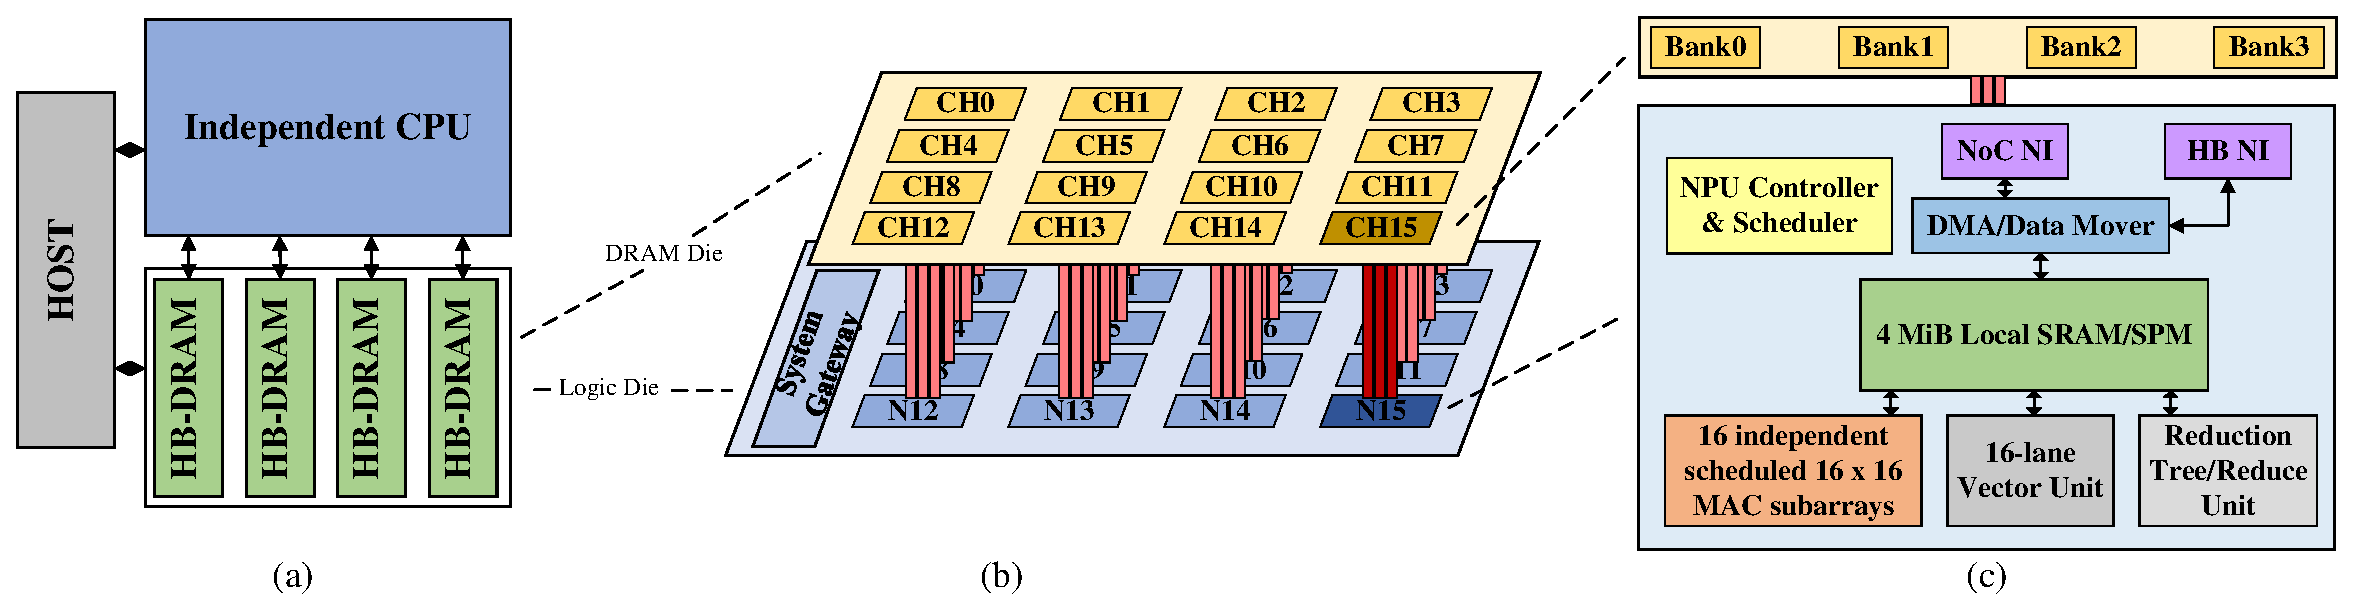
\includegraphics[width=\columnwidth]{figures/target_architecture.pdf}
  \caption{Target 3D system. (a) Host and HB-DRAM organization. (b) Face-to-face
  integration of the $4\times4$ Logic-tier NPU mesh and the aligned DRAM
  channels. (c) Microarchitecture of an NPU--memory pair.}
  \Description{Three panels show the host and HB-DRAM organization, the
  vertically aligned NPU clusters and DRAM channels, and the internal
  organization of one NPU--memory pair.}
  \label{fig:target-architecture}
\end{figure}

Figure~\ref{fig:target-architecture} shows a 3D accelerator in which the
logic and memory tiers are integrated by face-to-face hybrid bonding.
Each NPU cluster in the logic tier is vertically aligned with a DRAM
partition and accesses it through a local hybrid-bond link. A horizontal
$4\times4$ mesh NoC connects the NPU clusters and carries transfers between
them, including MoE dispatch and combine traffic. Local memory accesses and
inter-cluster transfers therefore use distinct physical paths. The vertical
alignment also couples the temperatures of the logic and DRAM tiers, so
concentrated activity in one tier can heat the other.

The main MoE evaluation covers Qwen3-30B-A3B~\cite{qwen3report} and
Qwen1.5-MoE-A2.7B~\cite{qwen15moe} for language-model inference,
mini-SWE-agent~\cite{minisweagent} with a Qwen3-30B-A3B backend for
SWE-bench Lite tasks~\cite{swebench}, and LingBot TI2V~\cite{lingbotvideo}
for video generation. The auxiliary thermal scenario combines
WHISPER~\cite{whisper}, an ORB-SLAM3-derived SLAM workload~\cite{orbslam3},
and $\pi_{0.5}$~\cite{pi05}.


\subsection{Phase-Dependent Congestion in MoE Communication}

\noindent\textbf{Problem.}
HiBand adapts communication locality by switching among four topologies---
Full-Local, Local-Biased, Global-Biased, and Full-Global---that repartition
bandwidth according to broad communication locality~\cite{wang2026hiband}.
MoE communication can concentrate transfers around a small set of busy NPU
nodes and links. When several messages need the same link or router output,
they must wait even if other parts of the network have spare capacity.
As hotspot locations change, the four predefined topologies may still leave
concentrated flows competing for the same links and router outputs, causing
persistent queueing despite spare capacity elsewhere.

Figure~\ref{fig:noc-phenomenon} shows the communication latency of
Qwen3-30B-A3B prefill. As input length increases
from 128 to 1024 tokens per request, the queueing share of mean network
round-trip latency rises from 57.2\% to 88.8\%, while mean zero-load latency
increases by 17.3\%. Zero-load latency includes serialization and traversal
without competing traffic; queueing is the additional delay under concurrent
traffic. Thus, queueing at shared network resources dominates the growth in
communication latency as input length increases.

\noindent\textbf{Root Cause.}
The gating network (Gate) selects a small set of experts for each token.
During Dispatch, token activations are sent to the NPU nodes holding those
experts; Combine returns the corresponding expert outputs. We define a flow
as the messages from one source NPU to one destination NPU within a single
communication phase. During Dispatch, when many tokens select the same experts, or several
frequently selected experts reside on the same NPU, transfers concentrate at
a small set of destinations. Flows whose routes overlap then compete for
shared links and router outputs, creating queueing hotspots. Thus, hotspot
formation depends on both the distribution of Gate selections and expert placement.
Our controlled Qwen3 decoding test also shows that concentrated accesses
can serialize requests at shared DRAM banks. Spreading those accesses across
banks addresses memory-side waiting, while overlapping NoC routes still
require path-level control.

Figure~\ref{fig:noc-cause} maps these messages onto deterministic XY paths.
Across MoE model layers 1, 24, and 48, the largest path-derived router demand
occurs at R9, R5, and R10, respectively. This spatial concentration can force multiple flows to share a
router output or link. Different concentrations can require different local
connections even when their total volume and aggregate communication locality
are similar. The design requirement is therefore to provide selectable local
paths around the contested resources, with explicit capacity at their
injection and receiving interfaces.

\begin{figure}[!tbp]
  \centering
  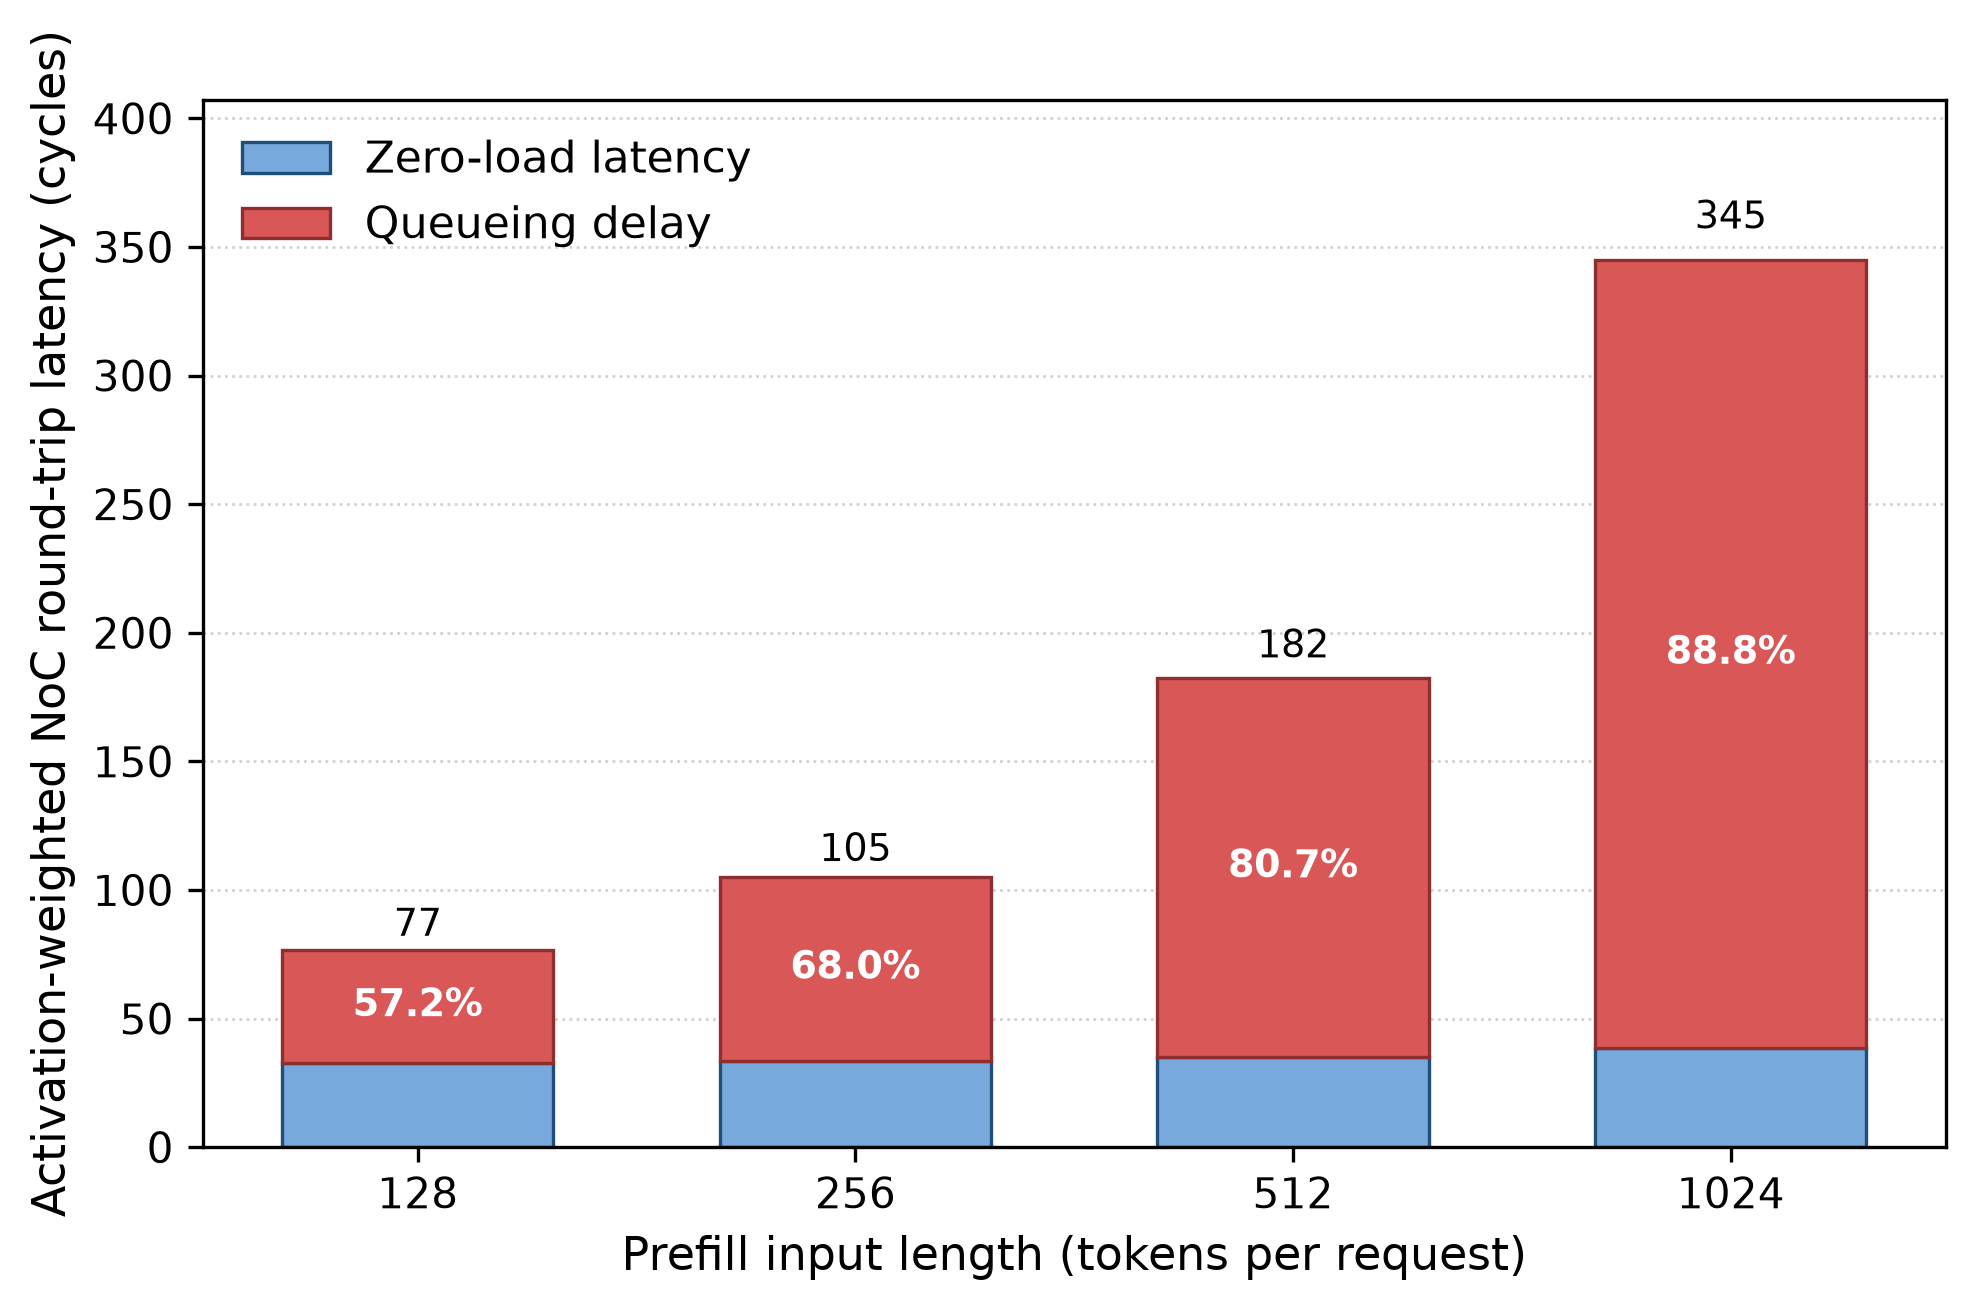
\includegraphics[width=\columnwidth]{figures/noc_phenomenon_input_tokens_0921.png}
  \caption{Qwen3-30B-A3B prefill communication on the fixed Mesh. Each bar
  reports the activation-weighted mean NoC round-trip latency at one input
  length. Zero-load
  latency contains serialization and uncongested traversal; queueing is the
  additional delay in the concurrent replay of the same message set. From 128
  to 1024 input tokens, the queueing share rises from 57.2\% to 88.8\%.}
  \Description{Four stacked bars for 128, 256, 512, and 1024 input tokens. The
  zero-load segment changes slightly, while the queueing segment grows rapidly
  and dominates the 1024-token bar.}
  \label{fig:noc-phenomenon}
\end{figure}

\begin{figure}[!tbp]
  \centering
  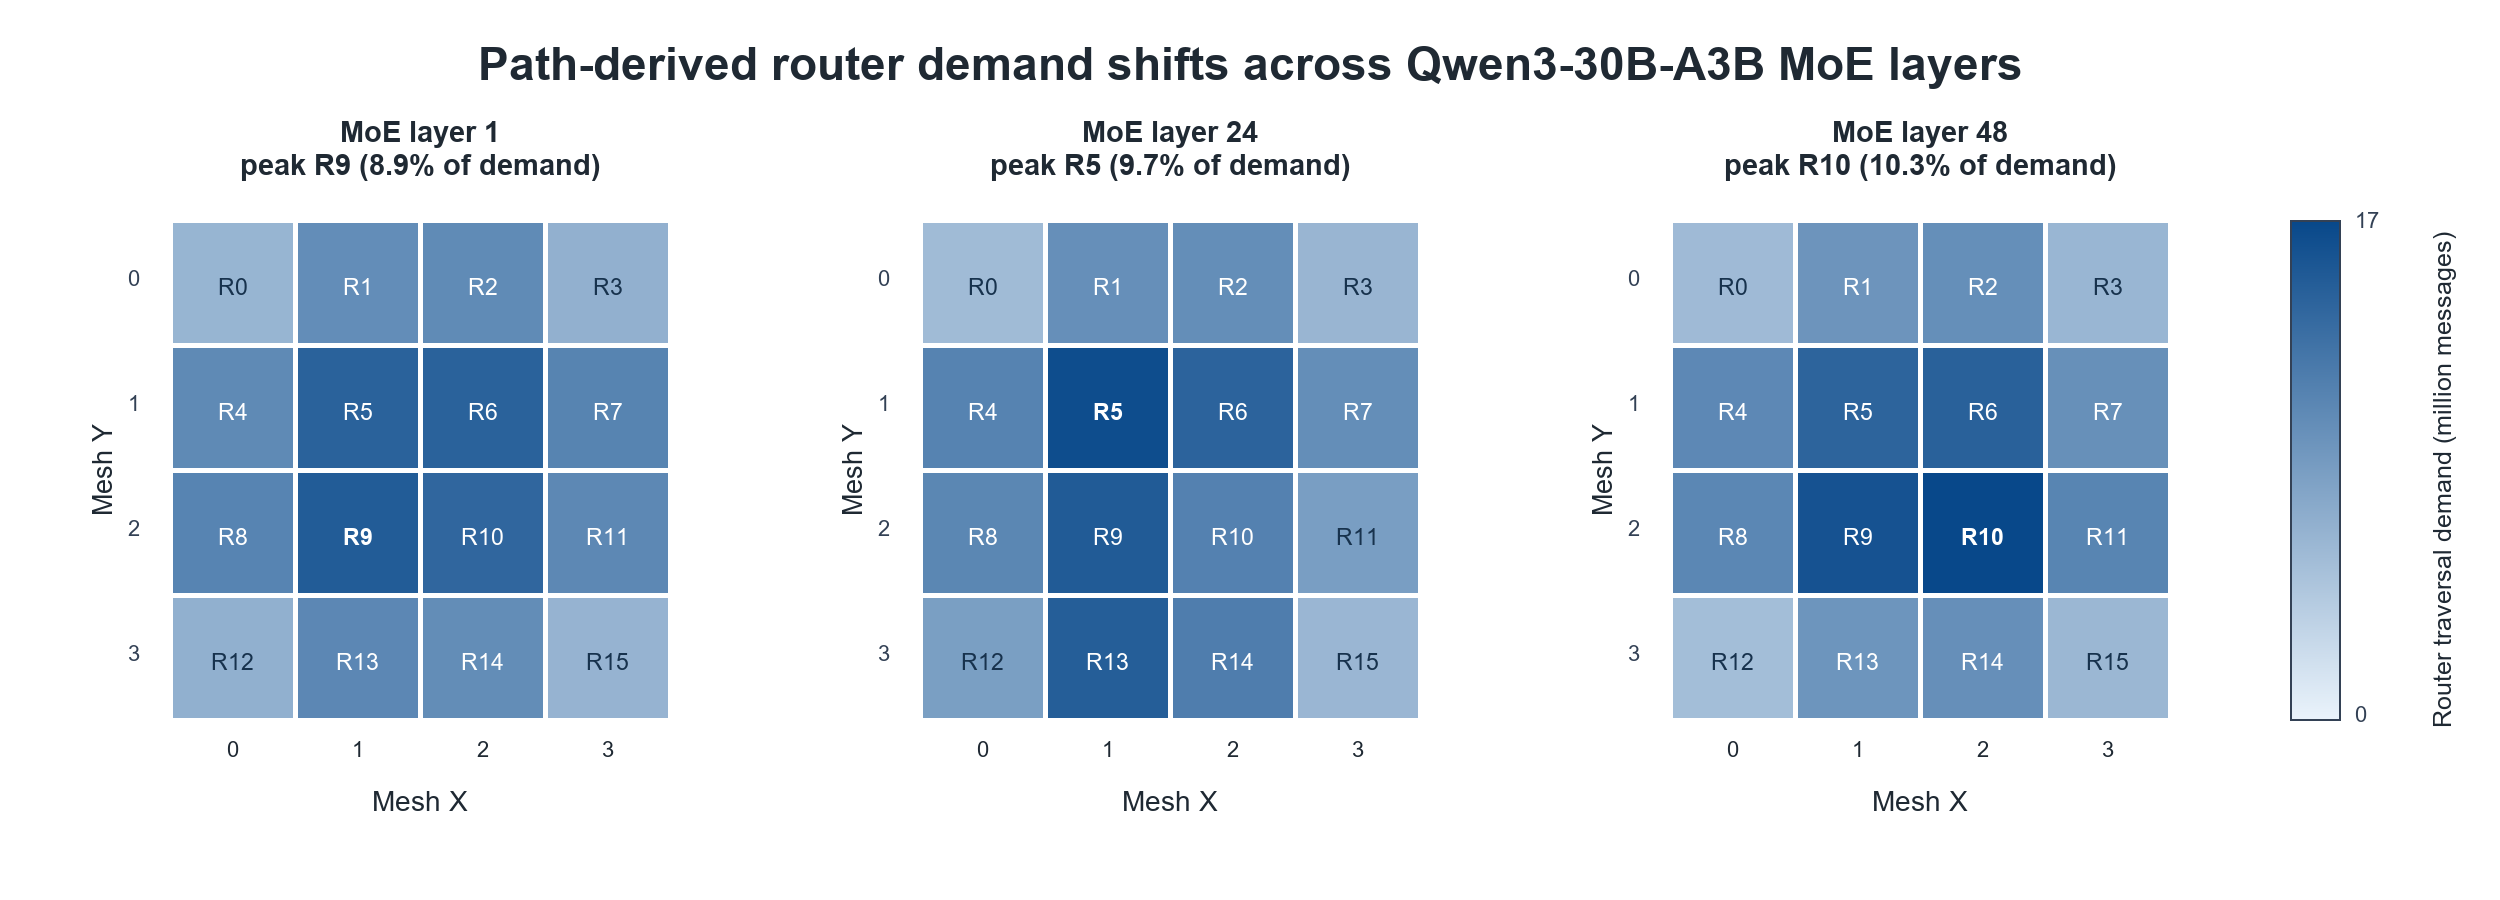
\includegraphics[width=\columnwidth]{figures/noc_cause_router_hotspots_revised.png}
  \caption{Path-derived router demand under the same Qwen3 trace. Each heatmap
  aggregates exact source--destination messages over every router on their
  deterministic XY path. With one shared scale, the peak moves
  R9$\rightarrow$R5$\rightarrow$R10 across
  MoE layers 1, 24, and 48, exposing a time-varying spatial demand pattern.}
  \Description{Three four-by-four router heatmaps for MoE layers 1, 24, and 48.
  The darkest cell changes location from router R9 to R5 and then R10.}
  \label{fig:noc-cause}
\end{figure}

\noindent\textbf{Opportunity: Configurable Local Connections.}
We place configurable switches (CSs) between neighboring NPU nodes in the same
Logic tier. Each switch selects connections between four fixed corner ports.
Using predicted hotspot locations, the controller configures nearby switches
to redirect selected transfers around congested links and router outputs,
and adjusts these connections as hotspot locations change. A selected
connection takes data from an auxiliary router output and delivers it directly
to the destination network interface (NI), bypassing intermediate Mesh routing
and the destination router's ordinary local output along that connection.
Traffic without a selected CS connection continues to use the Mesh.

Figure~\ref{fig:noc-opportunity} illustrates the mechanism. The XY route from
N2 to N5 traverses R2, R1, and R5. Switch C1 connects N1, N2, N5, and N6; setting
its northeast input to its southwest output permits the alternative
R2--C1--NI5 path. N2's transmit selector and N5's receive selector must both
select C1. This connection removes that transfer from the R1 path and R5 local
output and delivers the data to NI5's buffer-write interface.
When other messages compete for R1's output toward R5 or R5's local output,
diverting this transfer through C1 reduces the traffic using those outputs
and can relieve queueing.

\begin{figure}[!tbp]
  \centering
  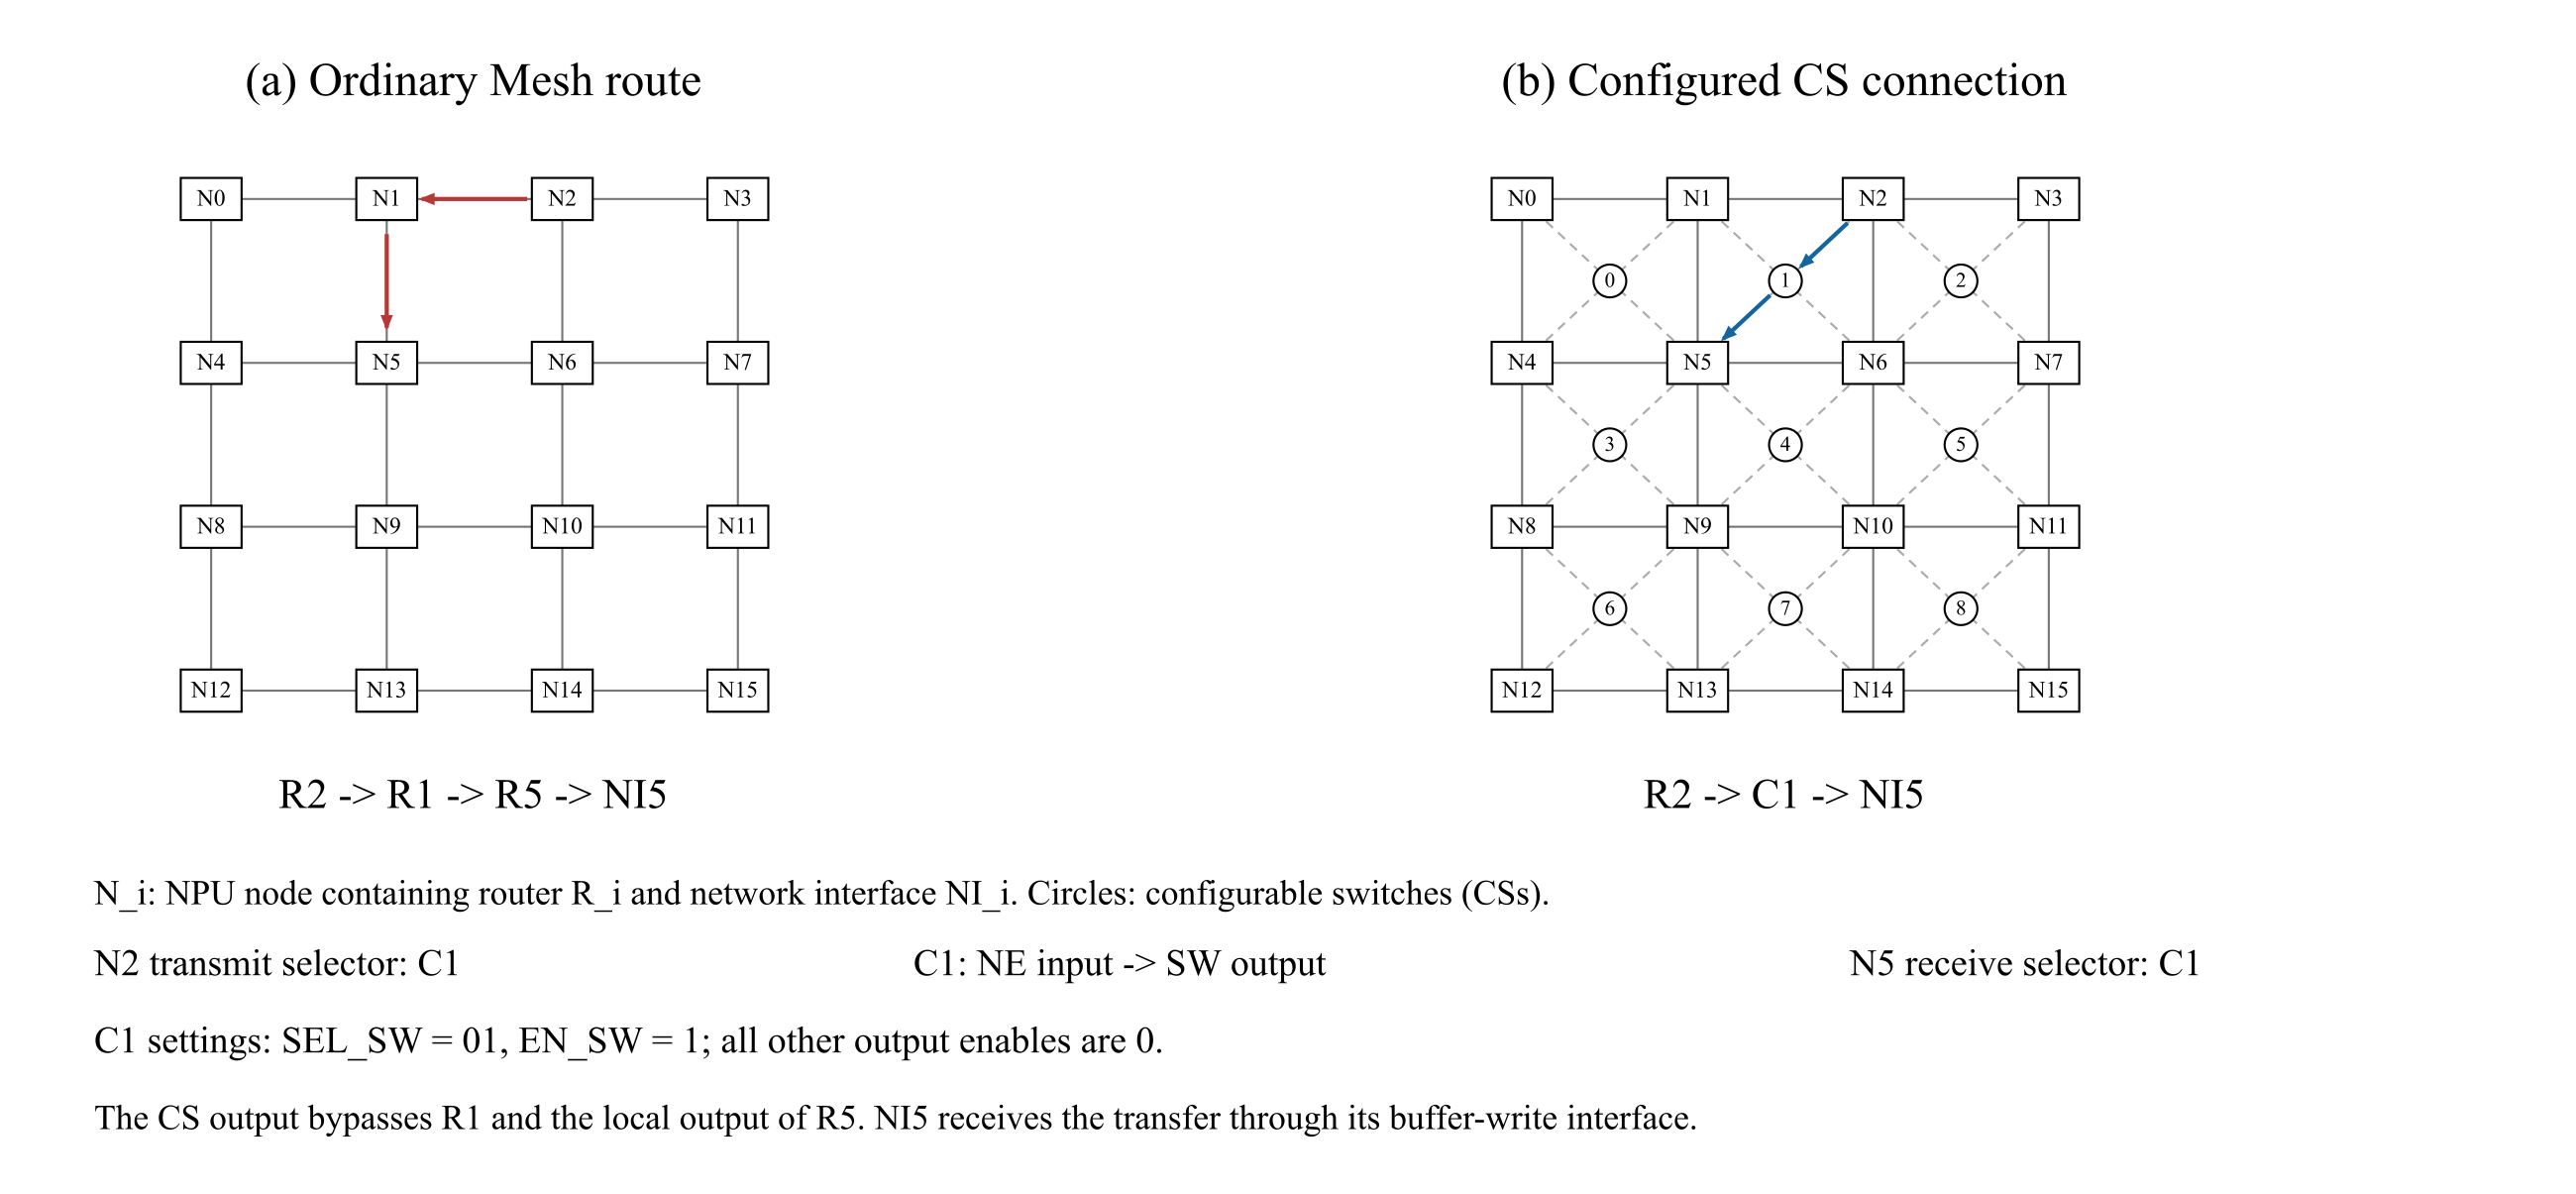
\includegraphics[width=\columnwidth]
  {figures/noc_opportunity_connection_example.png}
  \caption{Connection example for the NoC opportunity. (a) The ordinary
  N2-to-N5 route uses R1 and R5's local output. (b) A configured C1 connection
  delivers the transfer directly to NI5. The source transmit selector, CS
  connection, and destination receive selector are configured together.}
  \Description{Two four-by-four node layouts compare an ordinary Mesh route
  with a configured local-switch connection. A setting strip specifies N2 TX
  selection, the C1 northeast-to-southwest connection, and N5 RX selection.}
  \label{fig:noc-opportunity}
\end{figure}


Concentrating activity in a small region also affects the temperature of
both tiers. In our auxiliary thermal study, aligned logic and DRAM
hotspots persisted under AMBER-style thermal management~\cite{lin2026amber}.
This motivates using coupled temperature predictions to guide task
placement and regional DVFS.

\section{Design Directions}

\subsection{Memory-bank Design Directions}
\label{sec:bank-design}

Coaccess-aware page placement (CA) rearranges 4-KiB expert-weight pages
within each DRAM partition. From the historical development request
graphs, we group weight reads by DAG dependency depth within each
partition. Each pair of reads to different tensors in the same group
adds one to their coaccess weight. We apply that weight to page pairs
with matching offsets within those tensors. Dependency depth serves as
a proxy for concurrent demand.

Starting from a fixed layout, CA searches capacity-preserving page swaps
to reduce the total weight of pairs assigned to the same bank, breaking
ties by the sum of squared bank loads. Bank loads count profiled weight
reads for the pages assigned to each bank.


The runtime maps each logical weight page to a physical frame and
preserves its byte offset. CA remaps only read-only weight pages.
Mutable buffers retain their existing mappings. Moving a weight page
requires a source read and a destination write before the new mapping
takes effect. The evaluated layout assumes resident weights, with demand
paging outside the scope of this evaluation.

\subsection{Reconfigurable Local Connections for MoE Communication}
\label{sec:noc-design}

The NoC supplements the ordinary Mesh with configurable connections between
nearby NPU nodes. It redirects selected transfers away from congested Mesh
links and router outputs through configurable local connections that deliver
data directly to the destination NI. All data wires are fixed at fabrication.
Runtime control selects their input--output connections.

\noindent\textbf{Physical network and switch circuit.}
Figure~\ref{fig:noc-physical-design} separates the Mesh, the added connections,
and their combined placement in one Logic tier. The sixteen NPU nodes form a
$4\times4$ grid and are numbered from 0 to 15 in row-major order.
A configurable switch (CS) is placed within each adjacent $2\times2$ node
group, giving nine CSs. Let $r$ and $j$ denote the row and column indices of
a $2\times2$ node group, respectively, where $r,j\in\{0,1,2\}$.
The CS within that group is indexed by $c=3r+j$ and connects nodes
$4r+j$, $4r+j+1$, $4r+j+4$, and $4r+j+5$ at its NW, NE, SW, and SE
corners, respectively. NW, NE, SW, and SE denote
northwest, northeast, southwest, and southeast. CSs have no direct connections
to other CSs. A corner, edge, or interior node is adjacent to one, two, or four
CSs, respectively.

Each corner attachment comprises two separate directed data bundles: a router
auxiliary output to a CS input, and a CS output to the receiving NI. Each CS
contains four 3:1 output multiplexers (MUXes). An output selects one of the other three corner
inputs; selecting its own corner is excluded. Two selection bits and one enable
bit per output give a 12-bit CS configuration. SEL denotes input selection and
EN denotes connection enable. With output indices $o=0,1,2,3$ corresponding to
NW, NE, SW, SE, output $o$ uses selection bits $[3o+1:3o]$ and enable bit $[3o+2]$.
Selection codes 00, 01, and 10 index the other corners in that same order;
11 is unused. A disabled output has a zero configuration field. The selected
data and valid signal follow the same connection. The controller permits only
configurations in which each input is selected by at most one enabled output.

\begin{figure}[!tbp]
  \centering
  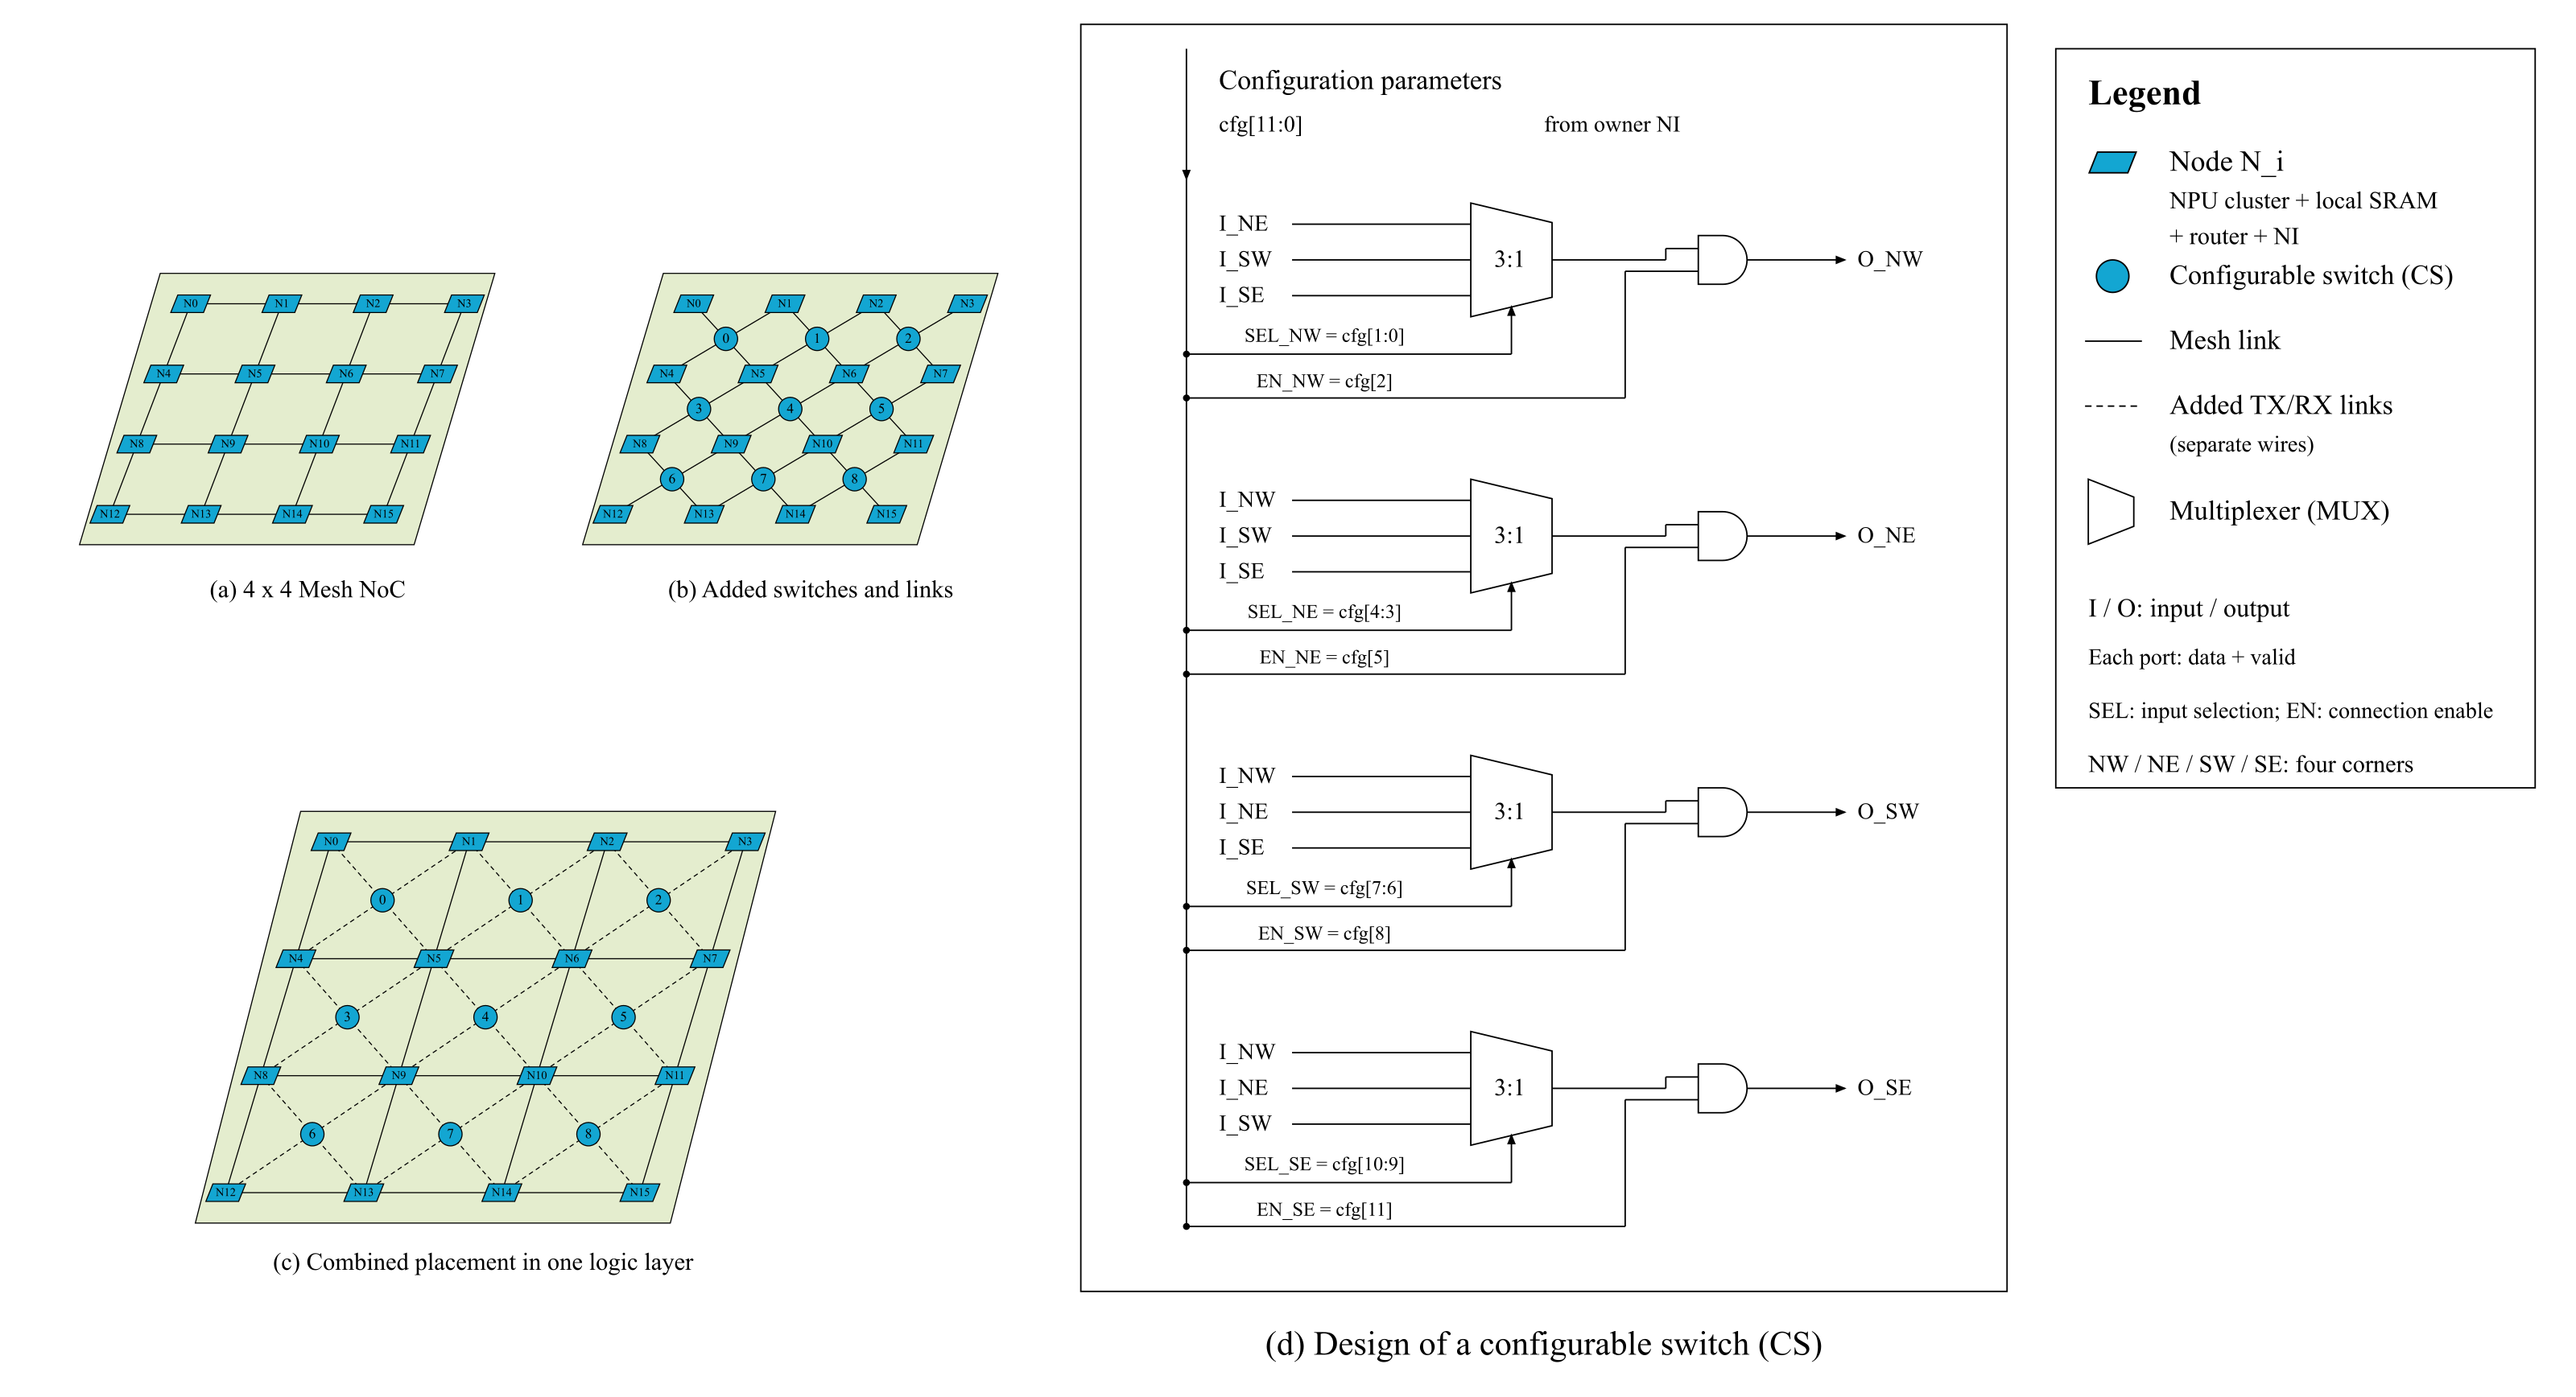
\includegraphics[width=\columnwidth]
  {figures/noc_ni_01_network_and_switch.png}
  \caption{Physical NoC organization. The Mesh, added corner attachments, and
  combined placement describe one network in the same Logic tier. Each CS
  contains four 3:1 MUXes with selection and enable inputs driven by the NI
  responsible for that CS. One drawn corner attachment represents separate transmit and receive
  data bundles.}
  \Description{Three aligned network views show the ordinary four-by-four
  Mesh, nine four-corner configurable switches, and their combined placement.
  A circuit inset expands the four output MUXes and their configuration bits.}
  \label{fig:noc-physical-design}
\end{figure}

\noindent\textbf{Router and NI attachment.}
Figure~\ref{fig:noc-node} shows a generic NPU node. The router retains its four
Mesh directions and local NI connection, and adds one auxiliary output.
A transmit selector sends that output to one adjacent CS. At the receiving
node, one receive selector chooses one adjacent CS output for the CS receive
first-in, first-out (FIFO) buffer inside the NI. The transmit and receive
selections are configured independently and remain fixed until the next
reconfiguration.

Ordinary traffic exits the destination router into the Mesh receive FIFO.
Auxiliary traffic reaches the CS receive FIFO without traversing that router's
local output. Both FIFOs feed the buffer-write interface and remain subject to
its arbitration, SRAM-bank availability, and backpressure. A credit advertises
one available FIFO entry. When an entry in the CS receive FIFO is freed,
the NI sends a credit pulse over separate reverse-control wires. The receive
selection routes the pulse to the selected CS, whose credit-return logic
uses the active SEL/EN configuration to route it back to the corresponding
input corner. The transmit selection then returns it to the transmitting
router's auxiliary credit counter. These control wires are separate from
the forward data MUXes. The transmit, CS, and receive selections remain
unchanged until the old transfers complete and their credits return.

For an auxiliary transfer from source $s$ to destination $d$, the controller
selects a forwarding node $g$ and CS $c$, where $g$ and $d$ are distinct corners of $c$.
The transfer first follows the deterministic Mesh route from $s$ to $g$, then uses
$g$'s auxiliary output, the configured CS connection, and $d$'s auxiliary
receive interface. When $g=s$, no intermediate Mesh link is needed. The data
packet carries destination $d$ and forwarding node $g$. Mesh routers forward
it toward $g$, whose auxiliary output uses the configured CS connection.

\begin{figure}[!tbp]
  \centering
  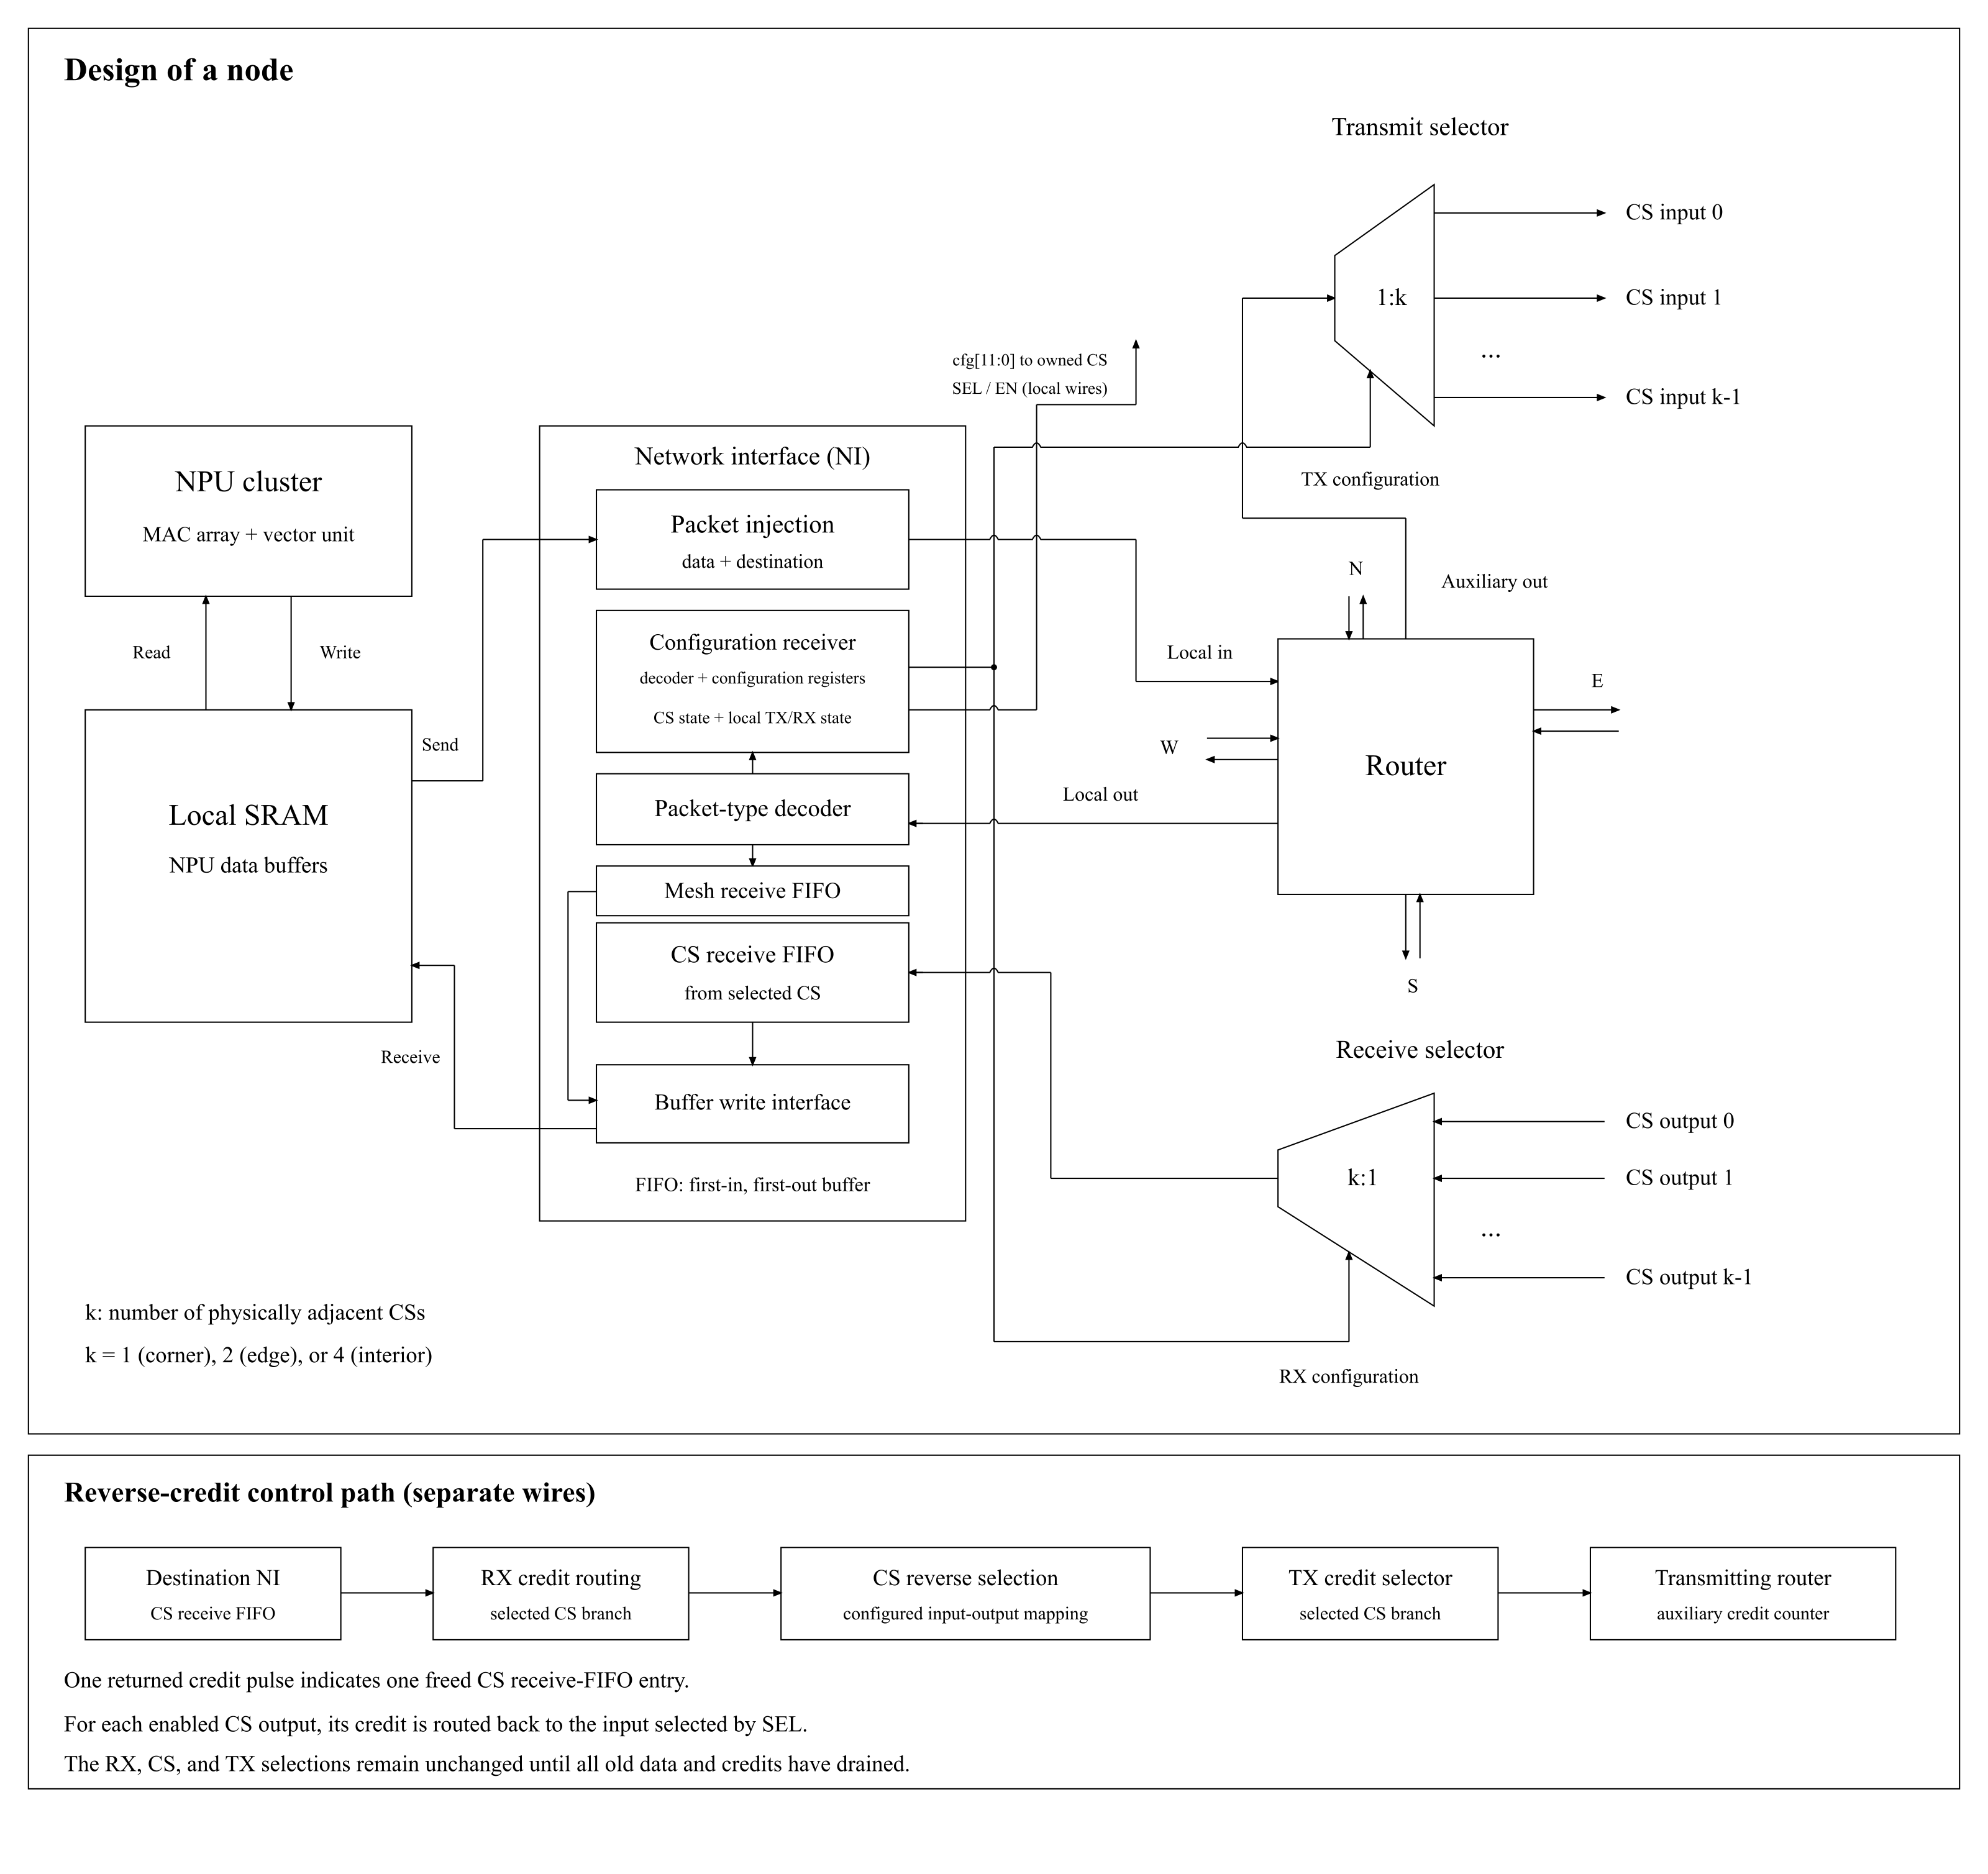
\includegraphics[width=\columnwidth]
  {figures/noc_ni_02_node_attachment_credit_1104.png}
  \caption{Design of an NPU node. The NI contains packet classification,
  configuration reception and storage, separate Mesh and CS receive FIFOs,
  and the local buffer-write interface. Its stored controls select one
  auxiliary transmit branch and one receive branch, and drive its owned CS.
  Separate reverse-control wires return credits from the CS receive FIFO
  through the configured RX, CS, and TX selections to the transmitting router.}
  \Description{An NPU cluster and local SRAM connect to the NI and Mesh router.
  Transmit and receive selectors attach the auxiliary interfaces to physically
  adjacent CSs. Configuration registers are contained in the NI. A lower
  inset shows the separate reverse-credit path from the receiving FIFO
  through the selected CS back to the transmitting router.}
  \label{fig:noc-node}
\end{figure}

\noindent\textbf{Obtaining communication demand.}
Configuration uses demand that is available before the affected messages are
injected. After the current Gate completes, the runtime groups token--expert
pairs by source and destination NPU. For one communication phase, let
$\mathcal F$ contain the inter-node flows with distinct source and destination
NPUs, and let $d_f$ be the actual
activation bytes of flow $f$. Dispatch volumes follow the current Gate result
and expert placement. Combine volumes follow the corresponding expert-output
and return-token relationships. Collective traffic follows the selected tensor
partition and collective algorithm, and is kept separate from these expert
flows when constructing the demand descriptors.

After Gate execution, the runtime sends the controller descriptors containing
the MoE model-layer index, communication phase, source NPU, destination NPU,
and byte count. The controller aggregates these descriptors and selects the
connection states before the phase's data injection. Aggregation, decision,
and configuration time are included in the execution timeline.

\noindent\textbf{Configuration problem.}
Let $\mathcal N=\{0,\ldots,15\}$ be the NPU-node set and
$\mathcal C=\{0,\ldots,8\}$ the CS set. The corner indices
$i,o\in\{0,1,2,3\}$ correspond to NW, NE, SW, and SE, respectively.
Let $v(c,i)$ be the node attached to corner $i$ of CS $c$, as defined by the
physical placement, and let $\mathcal C_n$ be the set of CSs adjacent to node $n$.
The binary variable $y_{c,i,o}$ equals one when the connection from input $i$
to output $o$ of CS $c$ is enabled. For $c\in\mathcal C_n$, the binary
variables $x^{\mathrm{TX}}_{n,c}$ and $x^{\mathrm{RX}}_{n,c}$ equal one when
node $n$ selects CS $c$ for auxiliary transmission and reception, respectively.
These variables form configuration $q=(y,x^{\mathrm{TX}},x^{\mathrm{RX}})$.
The physical connection constraints are
\begin{align}
 y_{c,i,i}&=0, & &\forall c,i,\label{eq:noc-no-return}\\
 \sum_i y_{c,i,o}&\leq1, & &\forall c,o,\label{eq:noc-output}\\
 \sum_o y_{c,i,o}&\leq1, & &\forall c,i,\label{eq:noc-input}\\
 \sum_{c\in\mathcal C_n}x^{\mathrm{TX}}_{n,c}&\leq1,
 & &\forall n\in\mathcal N,\label{eq:noc-node-tx}\\
 \sum_{c\in\mathcal C_n}x^{\mathrm{RX}}_{n,c}&\leq1,
 & &\forall n\in\mathcal N,\label{eq:noc-node-rx}\\
 y_{c,i,o}&\leq x^{\mathrm{TX}}_{v(c,i),c},
 & &\forall c,i,o,\label{eq:noc-tx-match}\\
 y_{c,i,o}&\leq x^{\mathrm{RX}}_{v(c,o),c},
 & &\forall c,i,o.\label{eq:noc-rx-match}
\end{align}
The first three constraints exclude same-corner returns and input or output
reuse within a CS. The next two enforce each node's single auxiliary transmit
and receive channels across all adjacent CSs. The last two require each
enabled CS connection to match the transmitting and receiving nodes' selectors.

For each flow $f\in\mathcal F$ from source $s$ to destination $d$, let
$\mathcal P_f$ contain its ordinary Mesh route and all candidate auxiliary
routes of the form $s\rightarrow g\rightarrow c\rightarrow d$, where
$g=v(c,i)$, $d=v(c,o)$, and $i\ne o$. The $s$-to-$g$ segment follows the
deterministic Mesh route. The binary variable $z_{f,p}$ equals one when the
entire flow uses candidate route $p\in\mathcal P_f$. The route constraints are
\begin{align}
 \sum_{p\in\mathcal P_f}z_{f,p}&=1, & &\forall f\in\mathcal F,
 \label{eq:noc-flow-route}\\
 z_{f,p}&\leq y_{c,i,o}, & &\forall f,\ p\in\mathcal P_f^{\mathrm{aux}},
 \label{eq:noc-route-match}
\end{align}
where $\mathcal P_f^{\mathrm{aux}}$ is the auxiliary-route subset of
$\mathcal P_f$, and $(c,i,o)$ identifies the CS connection used by route $p$.
Thus, each flow uses exactly one route without splitting its messages across
multiple paths. An auxiliary route can be selected only when its CS connection
and both node selectors are enabled consistently; the ordinary Mesh route
requires no CS connection. Let $\mathcal Q$ denote the set of all binary
configuration and route-assignment pairs $(q,z)$ satisfying these constraints.

Let $\mathcal E$ contain the resources used by these routes, including Mesh
links, ordinary router-local outputs, auxiliary channels, CS connections, and
NI buffer-write interfaces. Resource $e$ has service capacity $B_e$
in bytes per network cycle. Let $b_{f,p,e}$ be the bytes transmitted or written
by flow $f$ at resource $e$ when it takes route $p$. Link traffic includes packet headers
and flit padding, while a buffer-write interface counts the delivered activation
bytes. Packetization and the fixed route determine these quantities. The
aggregate demand is
\begin{equation}
 L_e(q,z)=\sum_{f\in\mathcal F}\sum_{\substack{p\in\mathcal P_f\\e\in p}}
 b_{f,p,e}z_{f,p}.
 \label{eq:noc-resource-demand}
\end{equation}
Serving $L_e$ bytes at capacity $B_e$ requires $L_e/B_e$ cycles. The objective
is to minimize the largest value across the resources used by the phase:
\begin{equation}
 \min_{(q,z)\in\mathcal Q}\Phi(q,z),\qquad
 \Phi(q,z)=\max_{e\in\mathcal E}\frac{L_e(q,z)}{B_e}.
 \label{eq:noc-serialization-demand}
\end{equation}
The shared NI write capacity is included in $\mathcal E$. Cycle-level
evaluation measures the resulting arbitration, queueing, and backpressure.

\noindent\textbf{Connection selection.}
Algorithm~\ref{alg:noc-reconfiguration} starts from the current configuration
and ordinary routes for the new phase. It evaluates physically adjacent
pairs of forwarding and destination nodes. A trial connection disables conflicting
connections that use the same transmit or receive channel, installs the new CS
connection and selector states, and returns any invalidated routes to the
ordinary Mesh. It then considers the affected destination's flows in descending
byte volume, breaking equal volumes by source and destination IDs, and assigns
a flow to the auxiliary route only if doing so reduces
$\Phi$. The trial is accepted only when its resulting $\Phi$ is lower than
that of the current solution. The comparison procedure Prefer ranks trials by
smaller $\Phi$, then fewer configuration-bit changes relative to
$q_{\mathrm{prev}}$, then smaller CS and node IDs. A configured iteration budget
$H$ bounds host-CPU work; the search also stops when no trial improves $\Phi$.
Here $t$ is the iteration index, $(q_b,z_b)$ is the best solution found in
the current iteration, and $(q',z')$ is a trial configuration and route assignment.

\begin{algorithm}[t]
\caption{Demand-Based CS Connection Selection}
\label{alg:noc-reconfiguration}
\begin{algorithmic}[1]
\Require phase flows $\mathcal F$, byte volumes $d_f$, fixed attachments,
  current configuration $q_{\mathrm{prev}}$, resource capacities $B_e$, iteration budget $H$
\Ensure feasible configuration $q$ and flow routes $z$
\Statex \Comment{Initialize connections and flow routes.}
\State $q\gets q_{\mathrm{prev}}$; $z\gets$ ordinary Mesh routes
\For{$t=1$ to $H$}
  \Statex \Comment{Retain the incumbent as this round's best.}
  \State $(q_b,z_b)\gets(q,z)$
  \ForAll{CSs $c$ and distinct corner nodes $g,d$ of $c$}
    \Statex \Comment{Remove conflicts; restore invalid routes to Mesh.}
    \Statex \Comment{Try affected flows in descending byte volume.}
    \State $(q',z')\gets\Call{TrialConnection}{q,z,c,g,d,\mathcal F}$
    \Statex \Comment{Rank by $\Phi$, bit changes, then IDs.}
    \If{\Call{Prefer}{$q',z',q_b,z_b,q_{\mathrm{prev}}$}}
      \State $(q_b,z_b)\gets(q',z')$
    \EndIf
  \EndFor
  \Statex \Comment{Stop if no trial strictly reduces $\Phi$.}
  \If{$\Phi(q_b,z_b)\geq\Phi(q,z)$}
    \State \textbf{break}
  \EndIf
  \Statex \Comment{Use the best trial in the next iteration.}
  \State $(q,z)\gets(q_b,z_b)$
\EndFor
\Statex \Comment{Return the selected connections and routes.}
\State \Return $(q,z)$
\end{algorithmic}
\end{algorithm}

TrialConnection performs the conflict removal and per-flow assignment
described above; all trials are checked against $\mathcal Q$. Selected routes
take effect after the configuration transition completes.
Traffic with no selected auxiliary route retains the ordinary Mesh path.
Configuration and transition time are reported together with the resulting
communication and application execution times.

\noindent\textbf{NI-based configuration.}
The independent host CPU executes the allocator and sends configuration
commands through the host gateway and existing Mesh. The NI of each CS's NW
adjacent node controls that CS. It performs packet-type classification,
target and state checks, and register updates. Both the pending and active
12-bit CS registers reside in that NI, as shown in
Figure~\ref{fig:noc-runtime-control}. The active register continuously drives
the adjacent CS's selection and enable inputs over fixed local control wires.
Each node's NI also stores the local transmit- and receive-selector
configurations. Configuration packets use the Mesh, and the NI's active
register drives the local CS control wires.

One configuration command contains 48 bits. Its 7-bit header contains the
3-bit Type and 4-bit destination-node ID. The remaining fields contain a 2-bit
Opcode, 2-bit Kind, 4-bit Target ID, 16-bit Epoch, 12-bit State, and five reserved
bits. Epoch is the configuration version; State contains the CS's SEL/EN
settings or the node-selector setting. Type 111 identifies configuration commands; Kind 00, 01, and 10 select a
CS, a node transmit selector, and a node receive selector. Opcode 00 is LOAD
and 10 is COMMIT. All operation and type codes are binary. For a node selector,
State[4] enables the connection and State[3:0] selects the adjacent CS ID;
State[11:5] is zero. COMMIT carries zero State, and the reserved bits are zero.
The header destination identifies the receiving NI, while
Target ID identifies its configuration object. The command occupies the upper
48 bits of one 256-bit flit, with zero padding in the remaining 208 bits.
Packet injection, router field extraction, and NI classification use this
control format consistently.

LOAD updates the NI's pending state without changing active connections.
Before COMMIT, the controller stops new auxiliary injection at all affected
nodes and waits for old transfers to complete and their credits to return. The NI accepts COMMIT
only for the matching pending epoch and copies the pending state into its
active register. Auxiliary traffic resumes after all affected modules confirm
the update and the local control signals have settled. Mesh traffic remains
available for configuration delivery during this interval.

\begin{figure}[!tbp]
  \centering
  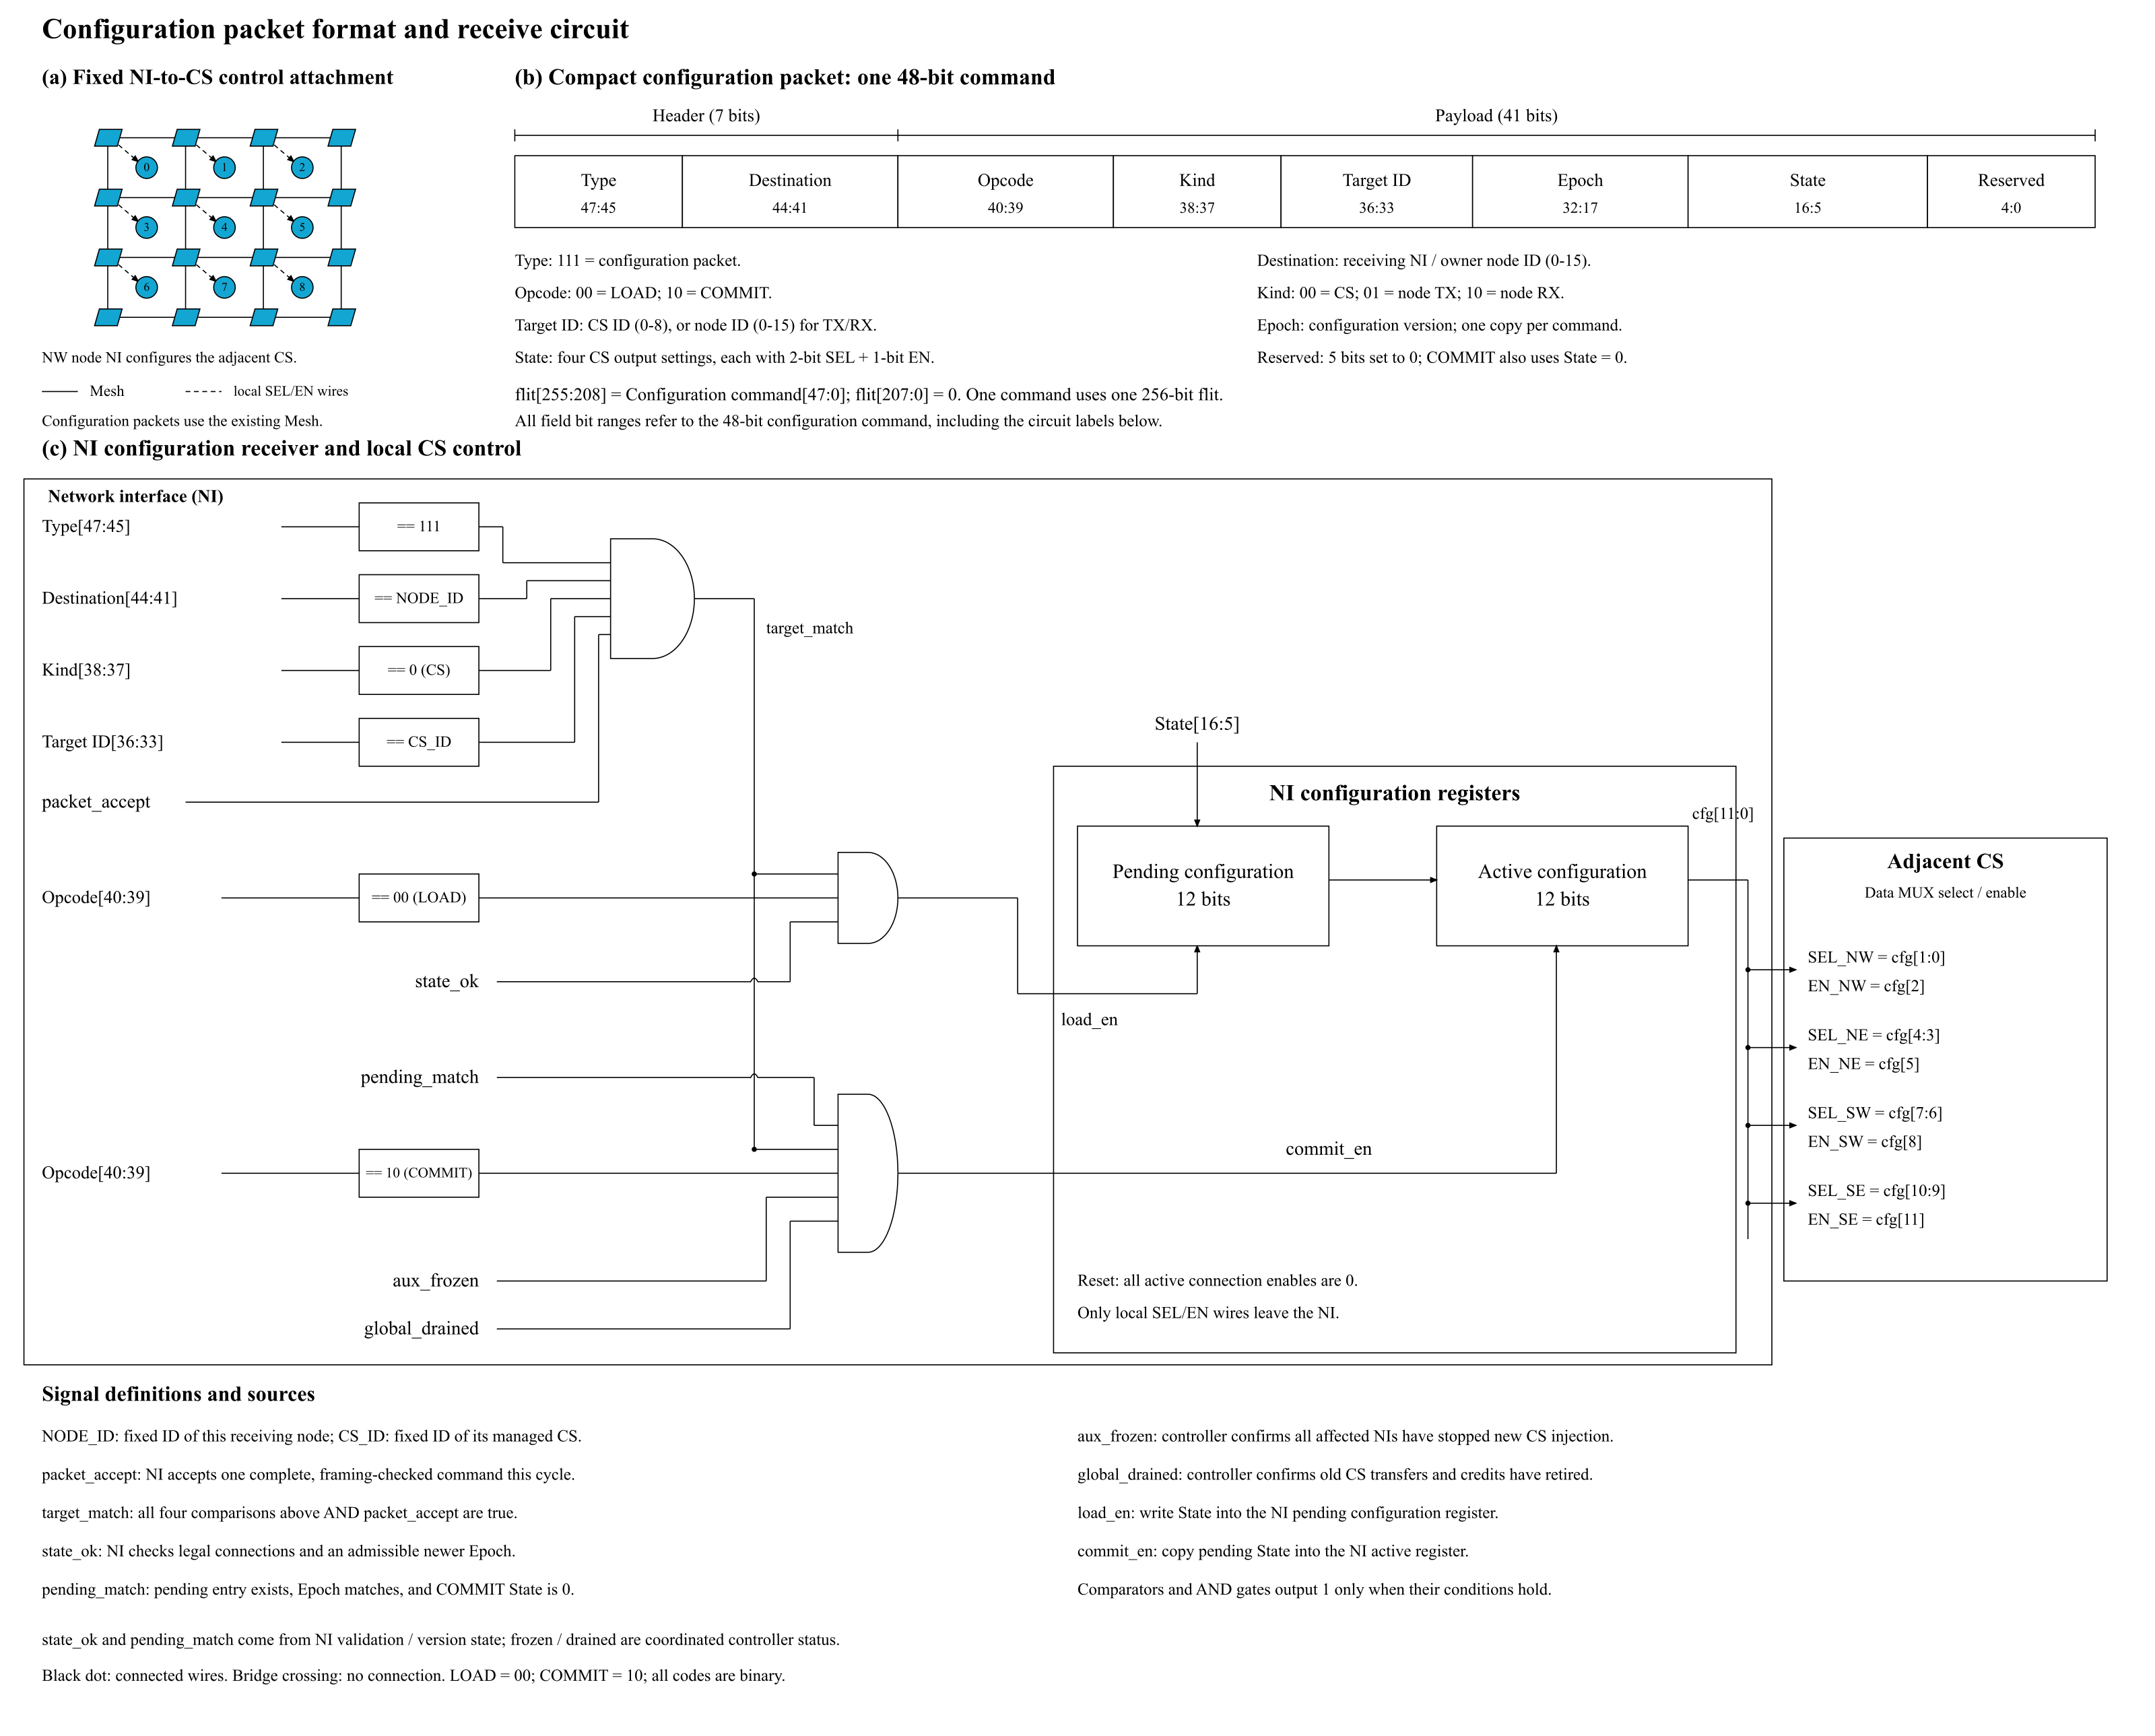
\includegraphics[width=\columnwidth]
  {figures/noc_ni_03_configuration_interface.png}
  \caption{NI-based configuration interface. Configuration commands travel
  over the Mesh to the NI responsible for the CS. Packet-field comparisons and LOAD/COMMIT
  conditions update the NI's pending and active registers; local SEL/EN wires
  connect the active state to the adjacent CS. The signal definitions identify
  the checks and coordinated stop/drain status used by the receive circuit.}
  \Description{A map of NI-to-CS control connections and a 48-bit command layout appear
  above the receive circuit. A large NI boundary encloses the comparisons and
  configuration registers. An adjacent CS outside that boundary receives the
  four groups of selection and enable signals.}
  \label{fig:noc-runtime-control}
\end{figure}



\subsection{Predictive Cross-Tier Thermal Management}
\label{sec:thermal-design}

Our controller selects where a ready task executes and at which
voltage--frequency setting. A location change redirects execution and
weight reads to a compute cluster with an existing local copy of the
required weights. Regional DVFS adjusts that cluster's power dissipation.
The controller evaluates both decisions using the coupled Logic--DRAM
thermal model before dispatch.
\noindent\textbf{Decision Variables and Objective.}
For task $i$, a candidate action is $a=(c,r)$, where $c$ is an eligible
NPU compute cluster, comprising a compute array and local SRAM.
The variable $r$ selects the cluster's frequency relative to the nominal
frequency and the corresponding voltage from the supported DVFS table.
The original-location plan $a_0$ provides a thermally safe reference.
An eligible cluster's associated DRAM partition must already contain
a complete copy of the required read-only weights, and the location
must satisfy the task's data-placement constraints. These existing
copies provide the alternative data sources considered during task
placement.

To compare temperature distributions across different tier floorplans,
we map both tiers onto $N=16$ common planar evaluation regions,
corresponding to the compute-cluster footprints in this architecture.
Let
$\mathcal{H}^{L}_k(a)$ and $\mathcal{H}^{D}_k(a)$ contain the hottest
$N/4$ regions in the predicted Logic and DRAM temperature maps at
step $k$. Each set therefore contains four regions, or the hottest
25\% of the evaluation regions in its tier. Their spatial overlap is
the number of regions shared by the two sets divided by four.
The predicted mean over a common $K$-step window is
\begin{equation}
  \widehat{\overline{O}}_{25}(a)=
  \frac{1}{K}\sum_{k=1}^{K}
  \frac{|\mathcal{H}^{L}_k(a)\cap\mathcal{H}^{D}_k(a)|}{N/4}.
  \label{eq:thermal-overlap-objective}
\end{equation}
The controller minimizes $\widehat{\overline{O}}_{25}(a)$ over feasible
candidates. Ties favor a lower positive spatial covariance between the
two temperature maps, accumulated over the same window, followed by
lower joint high-temperature exposure:
\begin{equation}
  D(a)=\sum_{k=1}^{K}\sum_{j=1}^{N}
  [\widehat{T}^{L}_{j,k}(a)-T_{\mathrm{target}}]_+
  [\widehat{T}^{D}_{j,k}(a)-T_{\mathrm{target}}]_+\Delta t,
  \label{eq:thermal-joint-exposure}
\end{equation}
where $[x]_+=\max(x,0)$ and $T_{\mathrm{target}}=80^\circ$C.
Each alternative must also satisfy $D(a)\leq D(a_0)$, checking absolute
high-temperature exposure alongside temperature ranking.

\noindent\textbf{Thermal State and Candidate Generation.}
The controller maintains the thermal RC state and the power
contributions of already scheduled tasks. Within each evaluation
region, the Logic temperature is the maximum of the CORE and SRAM
temperatures. The DRAM temperature is the maximum of the four DRAM
blocks whose planar footprints cover that region. The resulting maps
express the two temperature distributions in common planar coordinates.

The common scheduler selects the ready task and its reference plan.
The thermal controller searches alternatives when both tiers at the
original location exceed $T_{\mathrm{target}}$. It checks that the required
weight copies are present, prioritizes destinations outside the four
hottest DRAM evaluation regions, and then ranks them by the maximum
of their current Logic and DRAM temperatures.
At most two alternative destinations undergo thermal evaluation.
If the original location belongs to the hottest DRAM quarter, the
controller evaluates ratios $r\in\{0.5,0.75,1.0\}$; otherwise, it
retains the reference voltage--frequency setting during location selection.

\noindent\textbf{Candidate Timing, Power, and Temperature.}
Execution time and activity come from the profile for the selected
voltage--frequency setting. Input transfers use actual producer locations
and the NoC resource calendar, including transfer completion and queuing
delay. Computation, SRAM, DRAM, and communication activity generate
the spatial power trace. A HotSpot-derived RC model~\cite{hotspot_tool}
predicts the resulting 96-block temperature response at 1-ms intervals.
Candidates share the current thermal state and include outstanding
committed activities and background power. They are compared over
the same prediction window, covering execution and at least
128~ms of subsequent thermal response, together with the safety
lookahead.

\noindent\textbf{Feasibility and Selection.}
Thermal safety requires the predicted temperature of every block to
remain below $T_{\mathrm{limit}}-\delta$, with
$T_{\mathrm{limit}}=85^\circ$C and $\delta=1^\circ$C.
Candidate execution must preserve DAG dependencies, valid data
locations, the 32-GiB DRAM capacity, and the 4-MiB SRAM capacity per
cluster. Weight-copy eligibility includes address and profile compatibility;
tasks accessing writable KV state retain its required home.
The existing task-level Array/DMA reservations and link bandwidth
constraints remain part of scheduling.

We impose three policy budgets to contain the added execution and
resource costs. First, a candidate starts no later than the reference,
and its completion time satisfies
\begin{equation}
  e(a)\leq e(a_0)+\gamma d(a_0),\qquad \gamma=0.07,
  \label{eq:thermal-latency-budget}
\end{equation}
where $d(a_0)$ is the profiled execution time at the reference
operating point. Second, its input flow queuing delay is bounded
by the larger of the reference delay and the maximum previously
observed flow delay. Third, the maximum projected per-bank read/write
traffic cannot exceed the bound computed from the original full task
graph. This projection combines assigned tasks with the original
placement of remaining tasks.

Among feasible candidates, the controller accepts a lower predicted
overlap, or a lower covariance score when overlap is tied, subject to
the exposure constraint. If none qualifies, it retains the safe
original-location plan. When execution must wait for a thermally safe
start, previously committed activities continue and background power
contributes to the temperature evolution.

\noindent\textbf{Dispatch and Feedback.}
The selected plan commits the resource reservations and power events
used during prediction. Remapping updates the execution cluster,
weight-access partition, private workspace, and output location.
The selected task reads the existing weight copy at its destination.
Subsequent consumers obtain inputs from the actual producer location.
Running tasks and writable KV state retain their locations. Resource
availability and the thermal state are updated for the next decision.



\section{Evaluation Results and Analysis}
\label{sec:experiment}

\subsection{Experimental Setup}

We evaluate the proposed design on a face-to-face hybrid-bonded 3D accelerator. Table~\ref{tab:eval-platform} lists the common platform parameters. The evaluation uses 32~GiB of HB-DRAM. Each comparison starts from the same input and initial system state and uses the same precision, resource budget, and workload completion criteria. We account for each method's additional hardware and runtime costs separately.

\begin{table}[t]
\caption{Common hardware and simulation settings.}
\label{tab:eval-platform}
\centering\small
\begin{tabular}{@{}lp{0.59\columnwidth}@{}}
\hline
Component & Configuration \\
\hline
Logic tier & 16 NPU clusters at 1~GHz \\
NPU cluster & 4096 MACs, 16-lane vector unit, 4~MiB SRAM \\
Base NoC & $4\times4$ mesh, 256-bit links at 1~GHz \\
HB-DRAM & 32~GiB, 16 partitions of 2~GiB each, 16 logical banks per partition \\
Vertical link & 25.6~GB/s per NPU--memory pair \\
Host & Four CPU cores, PCIe 5.0, host memory xxx \\
Simulation & Compute, memory, and NoC models xxx \\
Thermal model & Ambient and initial temperatures xxx, temperature limit xxx \\
\hline
\end{tabular}
\end{table}

Table~\ref{tab:eval-workloads} lists four main MoE workloads and one auxiliary thermal scenario. We freeze the input manifests, arrival order, seeds, and stopping rules before collecting performance results.

\begin{table*}[t]
\caption{Workloads, input manifests, and measurement boundaries.}
\label{tab:eval-workloads}
\centering\small
\begin{tabular}{@{}lp{0.41\textwidth}p{0.30\textwidth}@{}}
\hline
Workload & Inputs and configuration & Measurement boundary \\
\hline
Qwen3-30B-A3B & Prompt source and IDs xxx, input/output lengths xxx, concurrency xxx & Prefill, decode, and complete request \\
Qwen1.5-MoE-A2.7B & Prompt source and IDs xxx, lengths xxx, TP/PP mapping xxx & Prefill, decode, and complete request \\
mini-SWE-agent + Qwen3 & SWE-bench Lite instance IDs and split xxx, tool and stopping rules xxx & Model calls, full agent task, and task outcome \\
LingBot TI2V & Text/image IDs xxx, resolution xxx, frames xxx, steps and seeds xxx & Encoding, denoising, scheduler, and VAE decoding \\
WHISPER + SLAM + $\pi_{0.5}$ & WHISPER version xxx, SLAM and $\pi_{0.5}$ traces xxx, request schedule xxx & Joint thermal scenario, execution coverage xxx \\
\hline
\end{tabular}
\end{table*}

For each experimental line, we first run the complete workload under both configurations and record stage latencies and the end-to-end critical path. Subsequent paired points measure the same one or two MoE layers with identical input and routing samples. We extrapolate both arms using the same layer selection, weights, and dependency model, including non-MoE stages and control costs. Recomputing the critical path preserves overlap among compute, memory, and communication. We validate the estimates against the complete runs and report measured layer latency, estimated end-to-end latency, and estimated speedup separately. The corresponding estimation errors are xxx. All reported execution times refer to the modeled target system.

\subsection{End-to-End Performance Comparison}

The primary comparison pairs the common platform baseline B with B plus the full design. We separately compare with prior methods that pass the same workload and timing checks under matched resource constraints. The HiBand reference implementation and other candidate NoCs enter this comparison after qualification. Table~\ref{tab:eval-comparisons} records the scope of each comparison.

\begin{table}[t]
\caption{Configurations and scope of the performance comparisons.}
\label{tab:eval-comparisons}
\centering\small
\begin{tabular}{@{}lp{0.53\columnwidth}@{}}
\hline
Configuration & Comparison scope \\
\hline
B & Common platform baseline, frozen configuration xxx \\
B + full design & Paired end-to-end comparison with B \\
HiBand reference & External comparison, qualification pending \\
Other NoC candidates & Configurations and qualification results xxx \\
\hline
\end{tabular}
\end{table}

Figure~\ref{fig:eval-overall} compares completion times for each main workload. For each pair, we compute the latency reduction as $1-T_{\mathrm{design}}/T_{\mathrm{ref}}$, where $T_{\mathrm{ref}}$ is the completion time of B or the named external comparator. We also report time to first token and time per output token for the language-model workloads. For mini-SWE-agent, we report model-call latency and task latency separately and record task outcomes. For LingBot, we report the latency of a complete generation. The measured end-to-end latencies, paired reductions, and workload-level exceptions are xxx.

\begin{figure*}[t]
\centering
\fbox{\rule{0pt}{18mm}\rule{0.92\textwidth}{0pt}}
\caption{End-to-end latency by workload for B, B plus the full design, and qualified external comparators. Each panel uses identical inputs and completion criteria. Labels distinguish complete-run measurements from estimates based on sampled MoE layers.}
\Description{Reserved space for the end-to-end latency comparison.}
\label{fig:eval-overall}
\end{figure*}

\subsection{Supporting Results and Thermal Ablation}

\paragraph{Phase-dependent congestion and bank waiting.}
To explain the latency differences in Figure~\ref{fig:eval-overall}, we trace matched MoE communication phases from memory requests through consumer readiness. We measure bank queueing before data becomes available, injection and router queueing, unloaded traversal, and synchronization at the slowest endpoint. We record configuration delay on the same timeline and attribute only exposed delays to the critical path. Comparing packet tails and router activity across phases tests whether a change in hotspot location translates into earlier consumer readiness. A comparison with fixed network policy and a bank-policy toggle can isolate the incremental effect of bank conflict mitigation. The paired changes in exposed waiting and packet tail latency are xxx.

\begin{figure*}[t]
\centering
\fbox{\rule{0pt}{17mm}\rule{0.92\textwidth}{0pt}}
\caption{Critical-path latency breakdown for matched MoE communication phases. The timeline shows bank service, data readiness, NoC injection and queueing, configuration, and consumer synchronization. Companion panels show packet tail latency and router activity using common scales across configurations.}
\Description{Reserved space for the critical-path breakdown and congestion panels.}
\label{fig:eval-breakdown}
\end{figure*}

\paragraph{Incremental effect of thermal management.}
We compare NoC with bank conflict mitigation and thermal management against the same NoC and bank mechanisms with thermal management disabled. Both arms start with identical temperatures, inputs, and thermal constraints. We track temperatures over the complete execution timeline and account for prediction, throttling, redistribution, and recovery where they occur. We report natural and thermally stressed scenarios separately. Peak temperature, time above the threshold, and completion time are xxx.

\begin{figure}[t]
\centering
\fbox{\rule{0pt}{17mm}\rule{0.90\columnwidth}{0pt}}
\caption{Temperature and workload progress with thermal management enabled and disabled. Both configurations use the same NoC and bank policies. Markers denote thermal triggers, throttling, and work redistribution where observed.}
\Description{Reserved space for temperature and workload progress curves.}
\label{fig:eval-thermal}
\end{figure}

\subsection{Scalability and Sensitivity Analysis}

We vary system scale and input scale separately. The system-scale sweep starts at 16 NPU clusters and holds workload fixed. At each scale, we report the topology, mapping, capacity, and bandwidth. The input-scale sweep fixes the platform and varies request concurrency or input size. We report absolute completion time and paired latency reduction at each point. To examine design sensitivity, we vary the local connection budget and reconfiguration interval one at a time and record completion time, packet tail latency, and exposed configuration cost. The tested ranges and observed trends are xxx.

\begin{figure}[t]
\centering
\fbox{\rule{0pt}{17mm}\rule{0.90\columnwidth}{0pt}}
\caption{Scalability and sensitivity. Panels show (a) system scale at fixed workload, (b) input scale at fixed system size, and (c) sensitivity to the local connection budget and reconfiguration interval. Markers indicate the default configuration and whether overall latency is measured or estimated.}
\Description{Reserved space for the scalability and parameter sweeps.}
\label{fig:eval-scale}
\end{figure}

\subsection{Hardware Cost and Runtime Overhead}

We report implementation costs for local switches, links and configuration logic, bank control, and thermal control. Table~\ref{tab:eval-cost} separates FPGA resource utilization, ASIC synthesis, and post-route results. Within each stage, baseline and enhanced implementations use the same tools and constraints. We state whether memories, physical interfaces, and cross-tier wiring are included and report module-level costs and system-level increments where available.

\begin{table}[t]
\caption{Hardware implementation cost by evaluation stage.}
\label{tab:eval-cost}
\centering\small
\begin{tabular}{@{}lp{0.63\columnwidth}@{}}
\hline
Stage & Conditions and reported results \\
\hline
FPGA prototype & Device/tool/clock xxx, LUT/FF/BRAM/DSP xxx, achieved frequency xxx \\
ASIC synthesis & Process/library/PVT/clock xxx, area xxx, power estimate xxx \\
Post-route ASIC & Extraction/PVT/activity xxx, area xxx, timing slack xxx, dynamic and leakage power xxx \\
\hline
\end{tabular}
\end{table}

Table~\ref{tab:eval-runtime} reports algorithm execution separately from the delay of applying its decisions. For each algorithm, we measure per-call time and call count, then report the fraction of total application latency exposed on the critical path. Configuration transfer, hardware reconfiguration, and thermal migration are accounted for as separate events.

\begin{table}[t]
\caption{Runtime overhead of online decision algorithms.}
\label{tab:eval-runtime}
\centering\small
\begin{tabular}{@{}lccc@{}}
\hline
Algorithm & Time/call & Calls & Exposed share \\
\hline
Hotspot prediction & xxx & xxx & xxx \\
Connection selection & xxx & xxx & xxx \\
Bank policy & xxx & xxx & xxx \\
Thermal control & xxx & xxx & xxx \\
\hline
\end{tabular}
\end{table}

\section{Related Works}
\label{sec:related-works}

\section{Conclusion}
\label{sec:conclusion}

\bibliographystyle{ACM-Reference-Format}
\bibliography{references,thermal_references}

\end{document}
